\chapter{Related Work}
\label{chap:related_work}

\section{Introduction}

Chapter~\ref{chap:compression} established the formal goal of quantization and pruning: to reduce bit-width, parameter counts, or computational costs, with bounded loss on the model's outputs. What remains is to decide how those goals are achieved in the context of large Transformers, particularly given the computational bottleneck described in Section~\ref{sec:transformer_bottleneck}, where size, structure, and deployment constraints determine which techniques are feasible. This chapter covers the main approaches taken.

Post-training quantization is reviewed from the perspective of precision reduction under activation outliers: the systematic high-magnitude activations that appear in large language models make uniform low-bit quantization lossy, and the methods reviewed here differ in how they handle that constraint, through weight rotation \cite{ashkboos2024quarot}, salience-aware protection \cite{lin2024awq}, or second-order weight adjustment \cite{frantar2022gptq}.

Pruning is reviewed along two paired dimensions: the topology of the sparsity produced, and the signal used to determine which units to drop. Both dimensions bear on deployment, since methods with similar compression ratios can correspond to very different runtimes and recovery costs.

% !TEX root = ../../main_without_quantization.tex

\providecommand{\methoddetail}[1]{%
  \par\medskip
  \noindent{\bfseries #1}\par
  \smallskip\noindent
}

\section{Related Work on Post-Training Quantization}

Post-training quantization has received considerable attention for large language models, where memory bandwidth is the dominant deployment cost and reducing bit-width directly lowers that cost without retraining. The discussion here is restricted to post-training methods — those that determine the quantized representation under limited post-training resources, without an additional training or fine-tuning phase. Quantization-aware training operates in a fundamentally different regime: it requires simulating quantization throughout a training or fine-tuning process, and its computational cost makes it unsuitable for LLMs at scale. OmniQuant notes that many LLM quantization methods specifically prioritize training-free PTQ for this reason \cite{shao2024omniquant}. Computationally efficient QAT variants still report 41 hours on a single A100-80GB for a 2-bit LLaMA-2-70B run \cite{tang2024efficientqat}, and standard QAT for 7B models requires more than 70GB of GPU memory \cite{bondarenko2024lrqat}. LLM-QAT makes the distinction concrete: quantization-aware training for LLMs is not a quantization formula but a full data-free distillation procedure over the pretrained model \cite{liu2023llm}, placing it in the same regime as recovery-based compression rather than post-training compression.

The methods reviewed here differ in how they control quantization error within the PTQ setting. The related work is organized by the dominant mechanism: rotation-based methods that redistribute activation energy before discretization, salience-based methods that identify and protect sensitive weights or channels, compensation-based methods that use second-order curvature to correct for quantization decisions locally, and optimization-based methods that tune quantization parameters directly on calibration data.

\subsection{Problem Setting and Taxonomy}

Post-train quantization (PTQ) reduces numerical precision after the full-precision phase. Conversion to lower bit-widths such as INT4 and INT8 lowers memory traffic and permits efficient integer arithmetic during inference. This makes PTQ particularly important for large language models, where deployment cost is often dominated by memory movement rather than arithmetic alone. Accuracy preservation, however, remains difficult. Moderate regimes typically focus on controlling layer-wise reconstruction error, whereas extreme regimes at $2$--$3$ bits must additionally address severe sensitivity to activation outliers and discrete approximation error \cite{frantar2022gptq,chee2024quip,ashkboos2024quarot}.

\begin{figure}[htbp]
  \centering
  \makebox[\textwidth][c]{%
    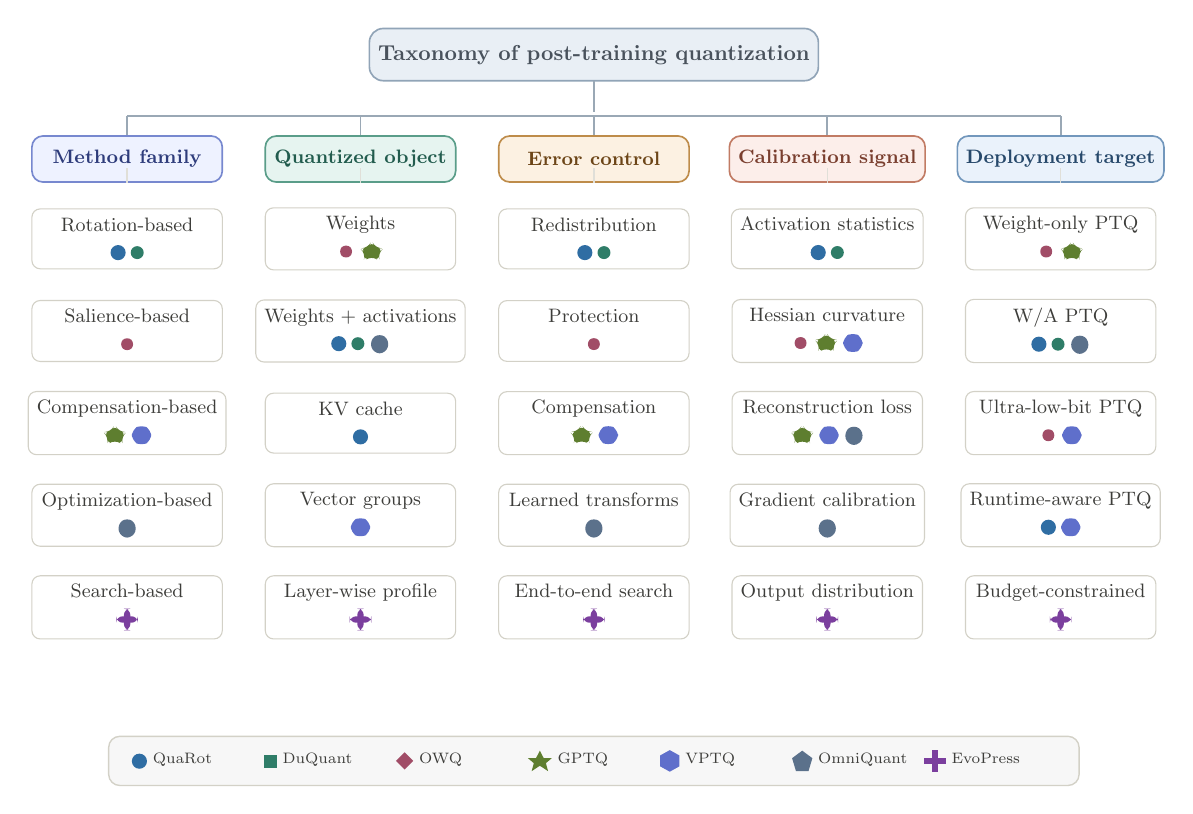
\begin{tikzpicture}[
  every node/.style={inner sep=4pt},
  font=\sffamily,
  scale=0.78,
  transform shape
]

\definecolor{rootbg}   {HTML}{E9EFF5}
\definecolor{rootbdr}  {HTML}{91A4B7}
\definecolor{trunkclr} {HTML}{9AA8B5}
\definecolor{leafbdr}  {HTML}{D3D1C7}
\definecolor{leaftxt}  {HTML}{3D3D3A}

\definecolor{ax1bg}  {HTML}{EEF2FF} \definecolor{ax1bd}  {HTML}{7788CF} \definecolor{ax1tx}  {HTML}{2E3C7B}
\definecolor{ax2bg}  {HTML}{E6F4F0} \definecolor{ax2bd}  {HTML}{5A9D89} \definecolor{ax2tx}  {HTML}{225C4E}
\definecolor{ax3bg}  {HTML}{FCF1E2} \definecolor{ax3bd}  {HTML}{BE8C4A} \definecolor{ax3tx}  {HTML}{6C4517}
\definecolor{ax4bg}  {HTML}{FCEEEA} \definecolor{ax4bd}  {HTML}{C17B64} \definecolor{ax4tx}  {HTML}{7A3F2F}
\definecolor{ax5bg}  {HTML}{EAF2FB} \definecolor{ax5bd}  {HTML}{7297BC} \definecolor{ax5tx}  {HTML}{27496B}

\definecolor{cquarot}  {HTML}{2F6DA3}
\definecolor{cduquant} {HTML}{2F7D68}
\definecolor{cowq}     {HTML}{A14D67}
\definecolor{cgptq}    {HTML}{5E7E2F}
\definecolor{cvptq}    {HTML}{5F6FCB}
\definecolor{comni}    {HTML}{5B718B}
\definecolor{cevopress}{HTML}{7B3F9E}

\newcommand{\symQuaRot}{\tikz[baseline=-1pt]\fill[cquarot] (0,0) circle (3.5pt);}
\newcommand{\symDuQuant}{\tikz[baseline=-1pt]\fill[cduquant] (-3pt,-3pt) rectangle (3pt,3pt);}
\newcommand{\symOWQ}{\tikz[baseline=-1pt]\fill[cowq] (0,4pt) -- (4pt,0) -- (0,-4pt) -- (-4pt,0) -- cycle;}
\newcommand{\symGPTQ}{\tikz[baseline=-1pt]
  \fill[cgptq] (0,5pt) -- (1.8pt,1.5pt) -- (5.5pt,1.5pt) -- (2.8pt,-0.8pt)
              -- (3.8pt,-4.5pt) -- (0,-2pt) -- (-3.8pt,-4.5pt)
              -- (-2.8pt,-0.8pt) -- (-5.5pt,1.5pt) -- (-1.8pt,1.5pt) -- cycle;}
\newcommand{\symVPTQ}{\tikz[baseline=-1pt]
  \fill[cvptq] (0,5pt) -- (4.5pt,2.5pt) -- (4.5pt,-2.5pt)
              -- (0,-5pt) -- (-4.5pt,-2.5pt) -- (-4.5pt,2.5pt) -- cycle;}
\newcommand{\symOmni}{\tikz[baseline=-1pt]
  \fill[comni] (0,5pt) -- (4.7pt,1.5pt) -- (2.9pt,-4.5pt)
              -- (-2.9pt,-4.5pt) -- (-4.7pt,1.5pt) -- cycle;}
\newcommand{\symEvoPress}{\tikz[baseline=-1pt]{
  \fill[cevopress] (-1.5pt,-5pt) rectangle (1.5pt,5pt);
  \fill[cevopress] (-5pt,-1.5pt) rectangle (5pt,1.5pt);}}

\def\rootY{0}
\def\trunkY{-1.0}
\def\headerY{-1.7}
\def\firstY{-3.0}
\def\rowstep{-1.50}

\def\xI{0}
\def\xII{3.8}
\def\xIII{7.6}
\def\xIV{11.4}
\def\xV{15.2}

\node[draw=rootbdr, fill=rootbg, rounded corners=5pt,
      minimum width=7.2cm, minimum height=0.85cm,
      font=\normalsize\bfseries\color{rootbdr!50!black},
      line width=0.6pt] at (7.6,\rootY) (ROOT) {Taxonomy of post-training quantization};

\draw[trunkclr, line width=0.7pt] (ROOT.south) -- ++(0,-0.5);
\draw[trunkclr, line width=0.7pt] (\xI,\trunkY) -- (\xV,\trunkY);
\foreach \cx in {\xI,\xII,\xIII,\xIV,\xV} {
  \draw[trunkclr, line width=0.7pt] (\cx,\trunkY) -- (\cx,\headerY+0.375);
}
\draw[trunkclr, line width=0.7pt] (7.6,\trunkY-0.5) -- (7.6,\trunkY);

% ---- Column 1: Method family ----
\node[draw=ax1bd, fill=ax1bg, rounded corners=4pt,
      minimum width=3.1cm, minimum height=0.75cm,
      font=\small\bfseries\color{ax1tx}, align=center,
      line width=0.6pt] at (\xI,\headerY) (H1) {Method family};
\draw[leafbdr!70, line width=0.5pt] (H1.south) -- ++(0, 5*\rowstep + 0.5cm);
\foreach[count=\i] \txt/\sym in {
  {Rotation-based}/{\symQuaRot\;\symDuQuant},
  {Salience-based}/{\symOWQ},
  {Compensation-based}/{\symGPTQ\;\symVPTQ},
  {Optimization-based}/{\symOmni},
  {Search-based}/{\symEvoPress}
}{
  \pgfmathsetmacro\ypos{\firstY + (\i-1)*\rowstep}
  \node[draw=leafbdr, fill=white, rounded corners=3pt,
        minimum width=3.1cm, minimum height=0.85cm,
        font=\small\color{leaftxt}, align=center,
        line width=0.4pt] at (\xI,\ypos) {\txt\\\footnotesize\sym};
}

% ---- Column 2: Quantized object ----
\node[draw=ax2bd, fill=ax2bg, rounded corners=4pt,
      minimum width=3.1cm, minimum height=0.75cm,
      font=\small\bfseries\color{ax2tx}, align=center,
      line width=0.6pt] at (\xII,\headerY) (H2) {Quantized object};
\draw[leafbdr!70, line width=0.5pt] (H2.south) -- ++(0, 5*\rowstep + 0.5cm);
\foreach[count=\i] \txt/\sym in {
  Weights/{\symOWQ\;\symGPTQ},
  {Weights + activations}/{\symQuaRot\;\symDuQuant\;\symOmni},
  {KV cache}/{\symQuaRot},
  {Vector groups}/{\symVPTQ},
  {Layer-wise profile}/{\symEvoPress}
}{
  \pgfmathsetmacro\ypos{\firstY + (\i-1)*\rowstep}
  \node[draw=leafbdr, fill=white, rounded corners=3pt,
        minimum width=3.1cm, minimum height=0.85cm,
        font=\small\color{leaftxt}, align=center,
        line width=0.4pt] at (\xII,\ypos) {\txt\\\footnotesize\sym};
}

% ---- Column 3: Error control ----
\node[draw=ax3bd, fill=ax3bg, rounded corners=4pt,
      minimum width=3.1cm, minimum height=0.75cm,
      font=\small\bfseries\color{ax3tx}, align=center,
      line width=0.6pt] at (\xIII,\headerY) (H3) {Error control};
\draw[leafbdr!70, line width=0.5pt] (H3.south) -- ++(0, 5*\rowstep + 0.5cm);
\foreach[count=\i] \txt/\sym in {
  Redistribution/{\symQuaRot\;\symDuQuant},
  Protection/{\symOWQ},
  Compensation/{\symGPTQ\;\symVPTQ},
  {Learned transforms}/{\symOmni},
  {End-to-end search}/{\symEvoPress}
}{
  \pgfmathsetmacro\ypos{\firstY + (\i-1)*\rowstep}
  \node[draw=leafbdr, fill=white, rounded corners=3pt,
        minimum width=3.1cm, minimum height=0.85cm,
        font=\small\color{leaftxt}, align=center,
        line width=0.4pt] at (\xIII,\ypos) {\txt\\\footnotesize\sym};
}

% ---- Column 4: Calibration signal ----
\node[draw=ax4bd, fill=ax4bg, rounded corners=4pt,
      minimum width=3.1cm, minimum height=0.75cm,
      font=\small\bfseries\color{ax4tx}, align=center,
      line width=0.6pt] at (\xIV,\headerY) (H4) {Calibration signal};
\draw[leafbdr!70, line width=0.5pt] (H4.south) -- ++(0, 5*\rowstep + 0.5cm);
\foreach[count=\i] \txt/\sym in {
  {Activation statistics}/{\symQuaRot\;\symDuQuant},
  {Hessian curvature}/{\symOWQ\;\symGPTQ\;\symVPTQ},
  {Reconstruction loss}/{\symGPTQ\;\symVPTQ\;\symOmni},
  {Gradient calibration}/{\symOmni},
  {Output distribution}/{\symEvoPress}
}{
  \pgfmathsetmacro\ypos{\firstY + (\i-1)*\rowstep}
  \node[draw=leafbdr, fill=white, rounded corners=3pt,
        minimum width=3.1cm, minimum height=0.85cm,
        font=\small\color{leaftxt}, align=center,
        line width=0.4pt] at (\xIV,\ypos) {\txt\\\footnotesize\sym};
}

% ---- Column 5: Deployment target ----
\node[draw=ax5bd, fill=ax5bg, rounded corners=4pt,
      minimum width=3.1cm, minimum height=0.75cm,
      font=\small\bfseries\color{ax5tx}, align=center,
      line width=0.6pt] at (\xV,\headerY) (H5) {Deployment target};
\draw[leafbdr!70, line width=0.5pt] (H5.south) -- ++(0, 5*\rowstep + 0.5cm);
\foreach[count=\i] \txt/\sym in {
  {Weight-only PTQ}/{\symOWQ\;\symGPTQ},
  {W/A PTQ}/{\symQuaRot\;\symDuQuant\;\symOmni},
  {Ultra-low-bit PTQ}/{\symOWQ\;\symVPTQ},
  {Runtime-aware PTQ}/{\symQuaRot\;\symVPTQ},
  {Budget-constrained}/{\symEvoPress}
}{
  \pgfmathsetmacro\ypos{\firstY + (\i-1)*\rowstep}
  \node[draw=leafbdr, fill=white, rounded corners=3pt,
        minimum width=3.1cm, minimum height=0.85cm,
        font=\small\color{leaftxt}, align=center,
        line width=0.4pt] at (\xV,\ypos) {\txt\\\footnotesize\sym};
}

% ---- Legend ----
\def\legY{-11.5}
\def\legXstart{0.0}
\def\legstep{2.15}

\draw[leafbdr, fill=white!97!black, rounded corners=4pt, line width=0.5pt]
  (-0.3,\legY-0.4) rectangle (15.5,\legY+0.4);

\foreach[count=\k] \sym/\lbl in {
  \symQuaRot/QuaRot,
  \symDuQuant/DuQuant,
  \symOWQ/OWQ,
  \symGPTQ/GPTQ,
  \symVPTQ/VPTQ,
  \symOmni/OmniQuant,
  \symEvoPress/EvoPress
}{
  \pgfmathsetmacro\lx{\legXstart + (\k-1)*\legstep}
  \node[font=\scriptsize\color{leaftxt}, anchor=west, inner sep=2pt]
    at (\lx,\legY) {\sym~\lbl};
}

\end{tikzpicture}
%
  }
  \caption[Taxonomy of post-training quantization methods]{Taxonomy of post-training quantization methods reviewed in this section.}
  \label{fig:type_of_ptq}
\end{figure}

The taxonomy organizes methods along five axes, summarized in Figure~\ref{fig:type_of_ptq}. The \textbf{method family} axis identifies the dominant error-control principle: rotation-based, salience-based, compensation-based, optimization-based, or search-based; each family is elaborated in the subsections that follow. The \textbf{quantized object} axis distinguishes weight-only, joint weight-and-activation, KV-cache, and vector-group compression regimes. The \textbf{error-control} axis captures the mechanism used to bound approximation error, from redistribution and protection to learned transforms and end-to-end search. The \textbf{calibration signal} records the informational basis used to set quantization parameters: activation statistics, Hessian curvature, reconstruction loss, gradient feedback, or output distribution. The \textbf{deployment target} axis links each formulation to its intended hardware outcome, whether storage reduction, bandwidth savings, full low-bit execution, or budget-constrained mixed-precision inference.


\subsubsection{Activation Outliers in Large Language Models}
\label{subsec:activation_outliers}
In the context of Large Language Models, quantization is fundamentally limited by the presence of \textit{outliers}, namely values with magnitudes significantly larger (often $100\times$) than the median distribution. Unlike standard statistical noise, outliers in Transformers exhibit a \textbf{systematic} structure: they appear persistently in specific feature channels across all tokens, a phenomenon that emerges as model scale increases (typically $>6$B parameters) \cite{dettmers2022llmint8}.

These outliers pose a critical challenge for uniform quantization. The scale $s$ in the affine mapping of Section~\ref{sec:quant_fundamentals} (Eq.~\ref{eq:quant_scale}) is fixed by the range endpoints, so under symmetric MinMax it reduces to $s = \max(|X|)/(2^k-1)$. A single massive outlier forces this range to stretch. Consequently, the vast majority of ``normal'' values are compressed into a minimal subset of available integers, causing catastrophic quantization error and performance collapse. The method families below differ mainly in how they prevent this single failure mode.


\subsection{Rotation-Based Methods}

The core challenge addressed by rotation-based methods is the presence of structured activation outliers in Transformer models. Prior work shows that Transformer activations can have high dynamic ranges and structured outliers, especially in residual streams, making them difficult to represent with low-bit fixed-point formats \cite{bondarenko2021understanding}. Subsequent studies show that these outliers are often concentrated in specific channels and may be asymmetric across channels, so a small number of activation dimensions can dominate the quantization range \cite{wei2023outlier+}. This behavior is also connected to architectural mechanisms inside Transformers: the LayerNorm scaling parameter has been identified as an amplifier of activation outliers, while attention and residual mechanisms have also been linked to the formation of strong outlier features \cite{wei2022outlier,bondarenko2023quantizable}. When activations are quantized naively, these large-magnitude channels determine the clipping or scaling range, leaving most non-outlier values compressed into a much smaller portion of the available quantization levels.

Rotation-based approaches address this issue using structured orthogonal transformations. Since an orthogonal matrix preserves the $\ell_2$ norm, rotating an activation vector does not change its total energy, but it redistributes that energy across coordinates. Methods such as QuaRot and SpinQuant exploit this property by inserting function-preserving rotations into Transformer blocks, reducing hidden-state outliers and improving low-bit quantization accuracy \cite{ashkboos2024quarot,liu2025spinquant}. In this sense, rotation does not remove information; it changes the coordinate system so that extreme channel-wise concentration becomes less harmful for uniform quantization.




\subsubsection{QuaRot \cite{ashkboos2024quarot}}

\begin{figure}[H]
  \centering
  \makebox[\textwidth][c]{%
    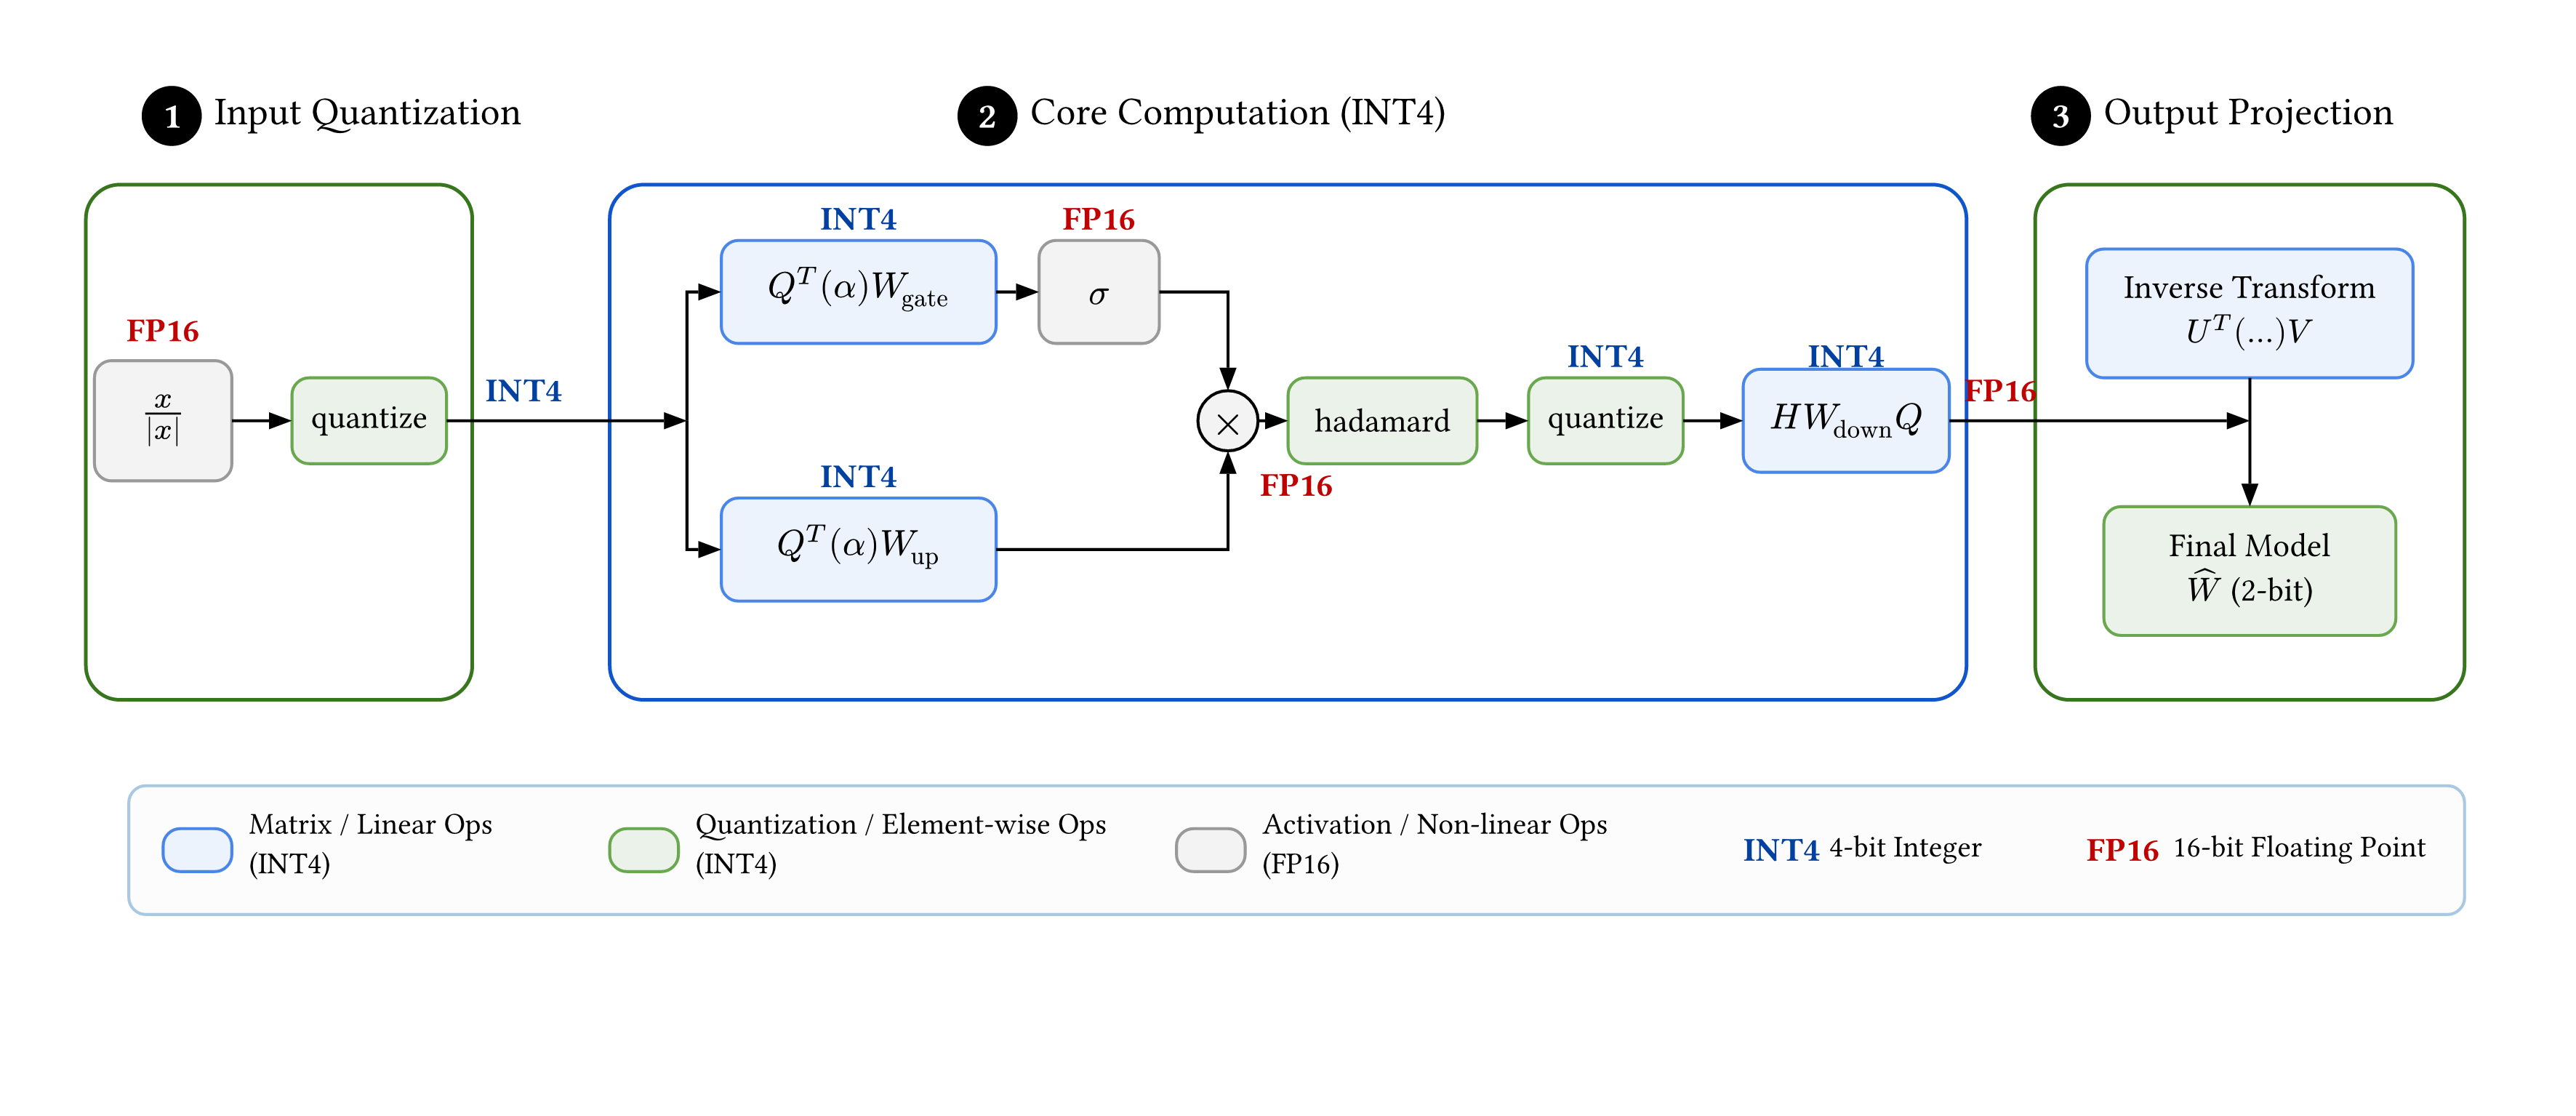
\includegraphics[width=0.98\textwidth,height=0.72\textheight,keepaspectratio]{figures/compression/quarot_pipeline.png}%
  }
  \caption[QuaRot FFN quantization pipeline]{QuaRot applied to a LLaMa-style FFN. RMSNorm scaling ($\alpha$) is absorbed into the weights. Hidden state $X$ is rotated by $Q$, canceled by $Q^\top$ in the first two weights. Weights and activations are INT4; matmul yields INT32, cast and scaled to FP16. While in FP16, a Hadamard transform is applied before quantizing and computing a modified down-proj, producing rotated output $YQ$. \cite{ashkboos2024quarot}}
  \label{fig:quarot}
\end{figure}

QuaRot introduces a quantization scheme based on randomized Hadamard rotations that eliminates activation outliers, enabling end-to-end 4-bit quantization of weights, activations, and the KV cache without performance degradation. Full 4-bit integer arithmetic is achieved by removing the root cause of quantization difficulty rather than working around it with mixed precision.

\paragraph{Methodology.}
The method relies on \textit{computational invariance} grounded in a basic property of orthogonal matrices: for any orthogonal $\bm{Q}$, $\bm{Q}\bm{Q}^\top = \bm{I}$, so inserting the pair $\bm{Q}^\top\bm{Q}$ between any two operations is an identity transformation. QuaRot exploits this to rotate activations by $\bm{Q}$ while multiplying $\bm{Q}^\top$ into the next weight matrix, leaving the computation unchanged but spreading outlier energy uniformly across channels before quantization. RMSNorm (Root Mean Square Normalization), which normalizes each token by the root mean square of its features, is compatible with this transformation: $\text{RMSNorm}(\bm{X}) = \text{RMSNorm}(\bm{X}\bm{Q}^\top)\bm{Q}$. The RMSNorm scaling parameters $\bm{\alpha}$ are first multiplied into the adjacent weights, then a randomized Hadamard matrix $\bm{Q}$ is multiplied into all input projections:
\begin{equation}
  \bm{W}_{in} \leftarrow \bm{Q}^\top \operatorname{diag}(\bm{\alpha})\, \bm{W}_{in}, \qquad \bm{X} \leftarrow \bm{X}\bm{Q},
  \label{eq:quarot_rotate}
\end{equation}
where $\bm{X}$ is the input activation matrix, $\bm{W}_{in}$ the weight matrices of input projections (query, key, value, and gate), and $\operatorname{diag}(\bm{\alpha})$ a diagonal matrix formed from the RMSNorm channel scales.
For the KV cache, per-head Hadamard matrices $\bm{H}_{d_h}$ are multiplied into the value and output projections to remove head-level outliers:
\begin{equation}
  \bm{W}_v \leftarrow \bm{W}_v(\bm{I} \otimes \bm{H}_{d_h}), \qquad \bm{W}_{\text{out}} \leftarrow (\bm{I} \otimes \bm{H}_{d_h})\bm{W}_{\text{out}},
\end{equation}
where $\bm{I}$ is the identity matrix, $\otimes$ denotes the Kronecker product that replicates $\bm{H}_{d_h}$ block-diagonally across all heads, and $d_h$ is the per-head dimension.
Within the FFN, a Hadamard $\bm{H}$ is applied during inference between the up- and down-projections and merged into the down-projection as $\bm{W}_{\text{down}} \leftarrow \bm{H}\bm{W}_{\text{down}}$. With outliers redistributed, weights are quantized to INT4 via GPTQ or RTN, activations are quantized per-token symmetrically during inference, and the KV cache uses asymmetric group-wise quantization.

\paragraph{Results.}
QuaRot yields up to $3.33\times$ prefill speedup and $3.89\times$ decoding memory savings on Llama-2-70B, with the 4-bit model retaining 99\% zero-shot performance and a perplexity increase of only 0.47 on WikiText-2.

\subsubsection{QuIP \cite{chee2024quip}}

\begin{figure}[H]
\centering
\makebox[\textwidth][c]{%
  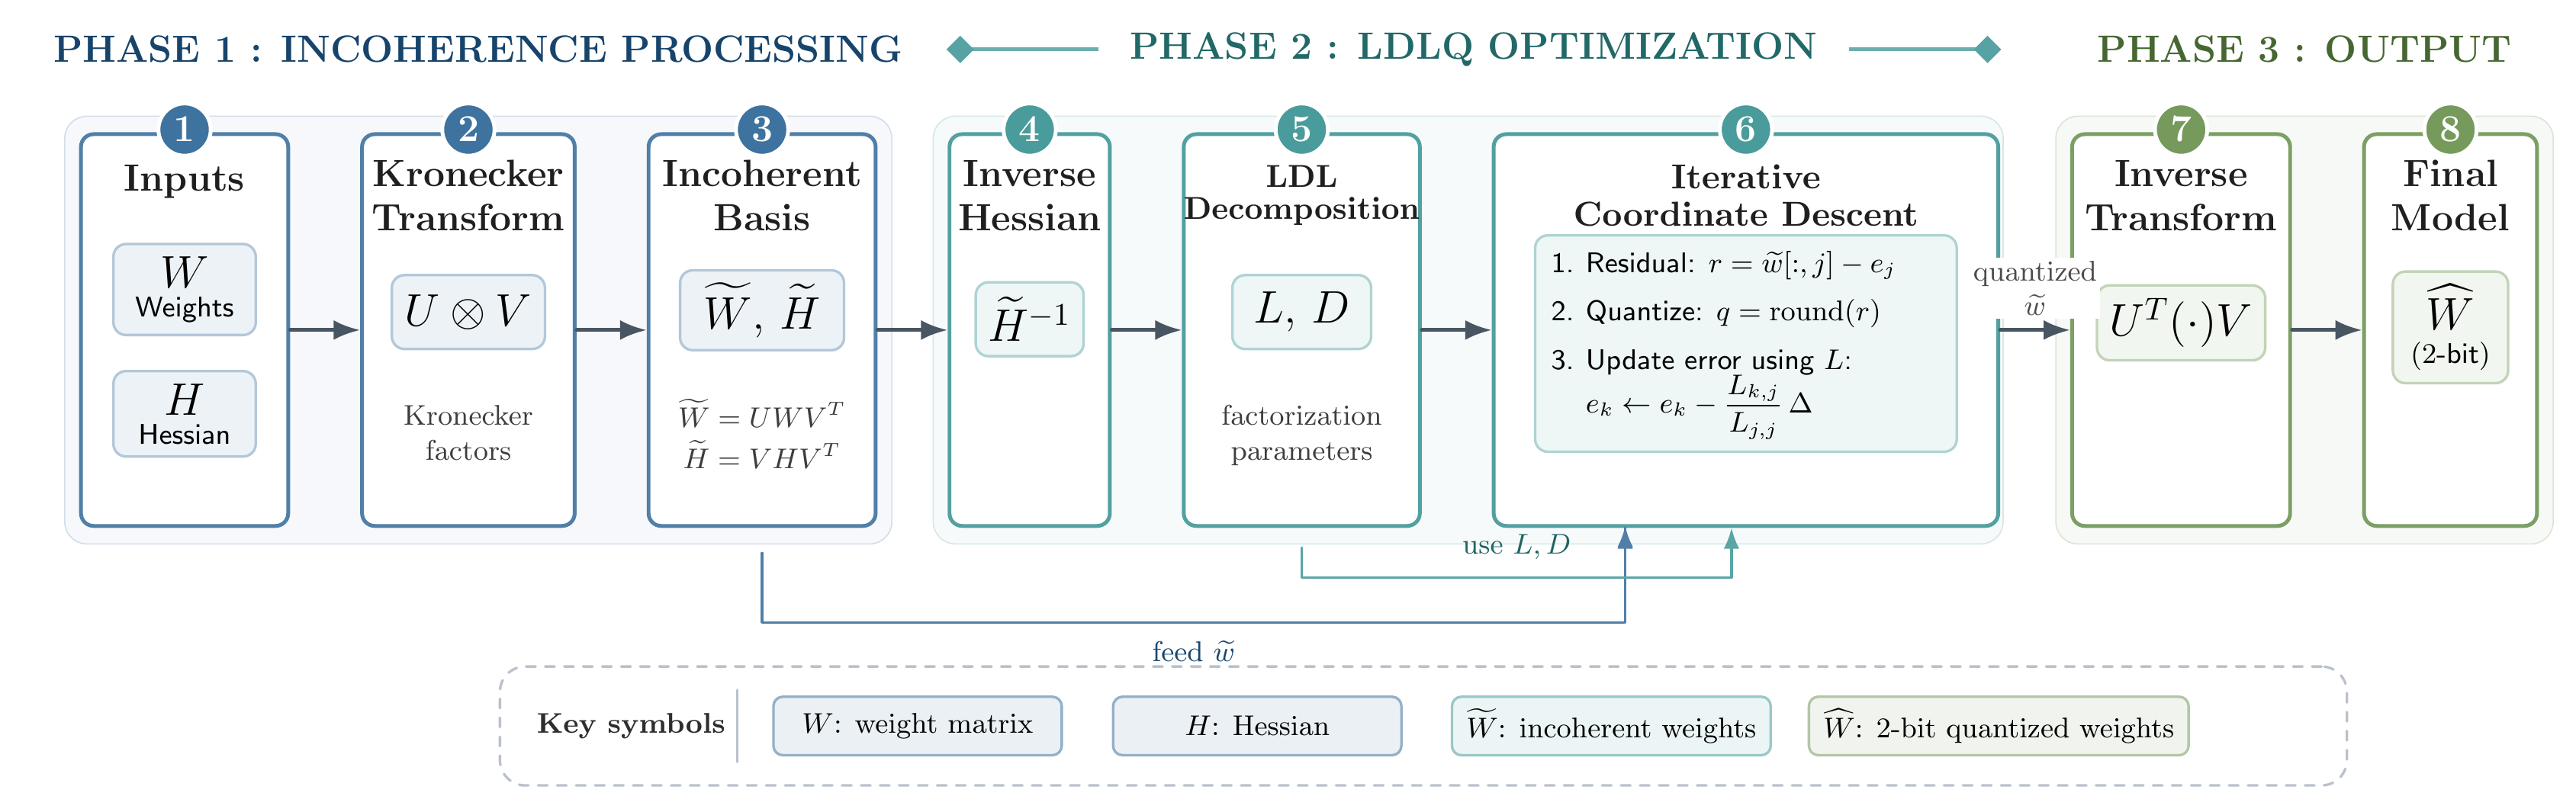
\includegraphics[width=0.98\textwidth,height=0.72\textheight,keepaspectratio]{figures/compression/quip_methodology.png}%
}
\caption[QuIP methodology]{QuIP Methodology. The approach tackles the "proxy gap" in 2-bit quantization by transforming the Hessian and weights into an incoherent basis using Kronecker-factored orthogonal matrices ($U$ and $V$), then employing LDLQ, a coordinate-descent algorithm using the $LDL^T$ decomposition of the inverse Hessian, to quantize weights while correcting errors in remaining full-precision weights. \cite{chee2024quip}}
\label{fig:quip_architecture}
\end{figure}

QuIP targets the ``proxy gap'' at 2-bit precision: the layer-wise quadratic proxy minimized by GPTQ correlates well with task loss at 4 bits but breaks down at 2 bits. The cause is that the LLM Hessian is coherent, with a few large eigenvalues dominating, so greedy quantization aligns error vectors with those principal directions and produces $O(d)$ worst-case error. QuIP addresses this by rotating weights and Hessian into an incoherent basis before quantization.

\paragraph{Methodology.}
Random orthogonal matrices $\bm{U} \in \mathbb{R}^{d_{\text{out}} \times d_{\text{out}}}$ and $\bm{V} \in \mathbb{R}^{d_{\text{in}} \times d_{\text{in}}}$ are applied as:
\begin{equation}
  \tilde{\bm{W}} = \bm{U}\bm{W}\bm{V}^\top, \qquad \tilde{\bm{H}} = \bm{V}\bm{H}\bm{V}^\top,
  \label{eq:quip_incoherence}
\end{equation}
where $\bm{V}$ spreads the Hessian eigenvalue spectrum so that no single direction dominates the quantization loss, $\bm{U}$ flattens weight magnitude distributions, and both matrices are Kronecker products of Hadamard matrices, keeping the transform cost $O(d \log d)$ rather than $O(d^2)$.

Quantization of the transformed weights $\tilde{\bm{W}}$ then proceeds via LDLQ (LDL$^\top$ Quantization), a coordinate-descent algorithm built on the $\bm{L}\bm{D}\bm{L}^\top$ factorization of $\tilde{\bm{H}}^{-1}$, where $\bm{L}$ is lower-triangular and $\bm{D}$ is diagonal. After rounding weight $j$ and collecting error $\delta_j = \tilde{w}_j - \hat{\tilde{w}}_j$, all future weights $k > j$ are corrected:
\begin{equation}
  \tilde{w}_k \leftarrow \tilde{w}_k - \frac{\bm{L}_{kj}}{\bm{L}_{jj}}\,\delta_j,
  \label{eq:quip_ldlq}
\end{equation}
where $\bm{L}_{kj}$ and $\bm{L}_{jj}$ are entries of $\bm{L}$ and $\delta_j$ is the scalar rounding error at column $j$. Operating on $\tilde{\bm{H}}^{-1}$ rather than $\bm{H}$ prevents outlier columns from propagating large corrections to later weights. Incoherence guarantees the proxy loss decreases at rate $O(1/n)$ in block size $n$, so error stays bounded rather than diverging as $n$ grows.

\methoddetail{Algorithm Overview}
QuIP quantizes each weight matrix in three steps and does not retrain the model. First, a pre-processing step rotates both the weight matrix and its Hessian into an incoherent basis by multiplying them with the random orthogonal matrices $\bm{U}$ and $\bm{V}$ (Eq.~\ref{eq:quip_incoherence}); in this basis the weight magnitudes are flattened and no single Hessian direction dominates, which is what makes rounding survive at 2 bits. Second, the rotated weights are quantized column by column with LDLQ: each column is rounded to the grid, and its rounding error is passed to the columns not yet quantized through the triangular factor $\bm{L}$ of the inverse Hessian, the same error-passing idea used by GPTQ (Eq.~\ref{eq:quip_ldlq}). Third, a post-processing step multiplies the quantized weights by $\bm{U}^\top$ and $\bm{V}$ to rotate them back into the original basis, so the stored low-bit matrix can be used directly at inference. Because $\bm{U}$ and $\bm{V}$ are products of small Hadamard matrices generated from a fixed random seed, they are cheap to apply and need not be stored.

\paragraph{Results.}
QuIP was the first method to produce non-degenerate output on LLaMA-2-70B at 2-bit precision, where GPTQ collapses entirely, and outperforms all prior 2-bit baselines on WikiText-2 perplexity across the LLaMA-1 and LLaMA-2 families.

\subsection{Salience-Based Methods}

Rotation-based methods reshape the activations so that one uniform grid fits every channel. The next family leaves the grid untouched and asks a different question: does every weight really deserve the same number of bits? The fundamental challenge addressed by salience-based methods is the heterogeneous importance of weights within neural networks. Not all parameters contribute equally to model output. Empirical analysis reveals that approximately $1\%$ of weights in Large Language Models are disproportionately critical for performance preservation, while the vast majority exhibit high redundancy. Uniform quantization schemes that apply identical bit-widths across all parameters fail to exploit this structure. They either misallocate precious bits on unimportant weights or catastrophically degrade salient features.

Salience-based approaches address this challenge through precision allocation according to importance. The core principle involves the preservation of high-impact weights with higher precision alongside aggressive quantization of low-impact parameters to minimal bit-widths. The critical technical question becomes: how to accurately measure ``importance'' in a post-train setting without access to gradients or optimization dynamics? Different methods answer this question differently; some rely on activation magnitude analysis, while others utilize Hessian-based sensitivity measures. However, all share the objective to align bit allocation with functional impact.

\subsubsection{OWQ \cite{lee2024owq}}

\begin{figure}[htbp]
\centering
\makebox[\textwidth][c]{%
  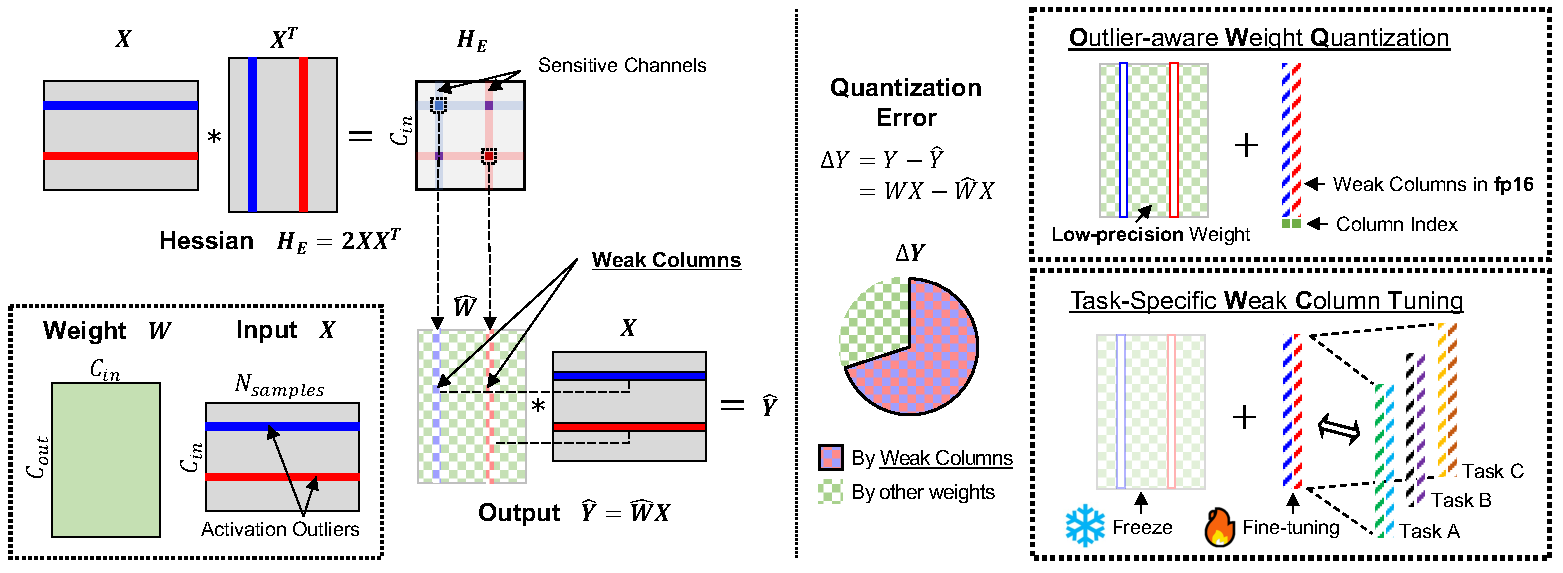
\includegraphics[width=0.98\textwidth,height=0.72\textheight,keepaspectratio]{figures/compression/owq_overview.pdf}%
}
\caption[OWQ overview]{Overview of OWQ (Outlier-Aware Weight Quantization). The method identifies ``weak columns'' in weight matrix $\bm{W}$ corresponding to outlier activation channels. These columns are segregated into sparse FP16 matrix $\bm{W}_{\text{weak}}$, while remaining ``strong columns'' are quantized to low precision using GPTQ. \cite{lee2024owq}}
\label{fig:owq}
\end{figure}

OWQ addresses the amplification problem inherent in quantizing weights that interact with outlier activations. Since output error is defined by $\Delta \bm{Y} = \Delta \bm{W} \bm{X}$, when $\bm{X}$ contains the outlier channels described in Section~\ref{subsec:activation_outliers} (magnitudes around $100\times$ larger than surrounding features), even small weight quantization errors $\Delta \bm{W}$ in the corresponding columns are amplified dramatically. Standard methods either clip activations (permanently destroying information needed for difficult reasoning) or apply uniform quantization (causing performance collapse). OWQ provides a principled mixed-precision solution based on Hessian sensitivity analysis.

\paragraph{Methodology.}
OWQ formulates weight importance through the expected output error variance:
\begin{equation}
\min_{\hat{\bm{W}}} \mathbb{E}\left[ \| (\bm{W} - \hat{\bm{W}})\bm{X} \|_2^2 \right] = \text{Tr}\left( (\bm{W} - \hat{\bm{W}})^\top (\bm{W} - \hat{\bm{W}}) \mathbb{E}[\bm{X}\bm{X}^\top] \right)
\end{equation}
The term $\mathbb{E}[\bm{X}\bm{X}^\top]$ forms the empirical Hessian $\bm{H}$. Error contribution of the $i$-th weight column is proportional to $\bm{H}_{ii}$ (the aggregate power of the $i$-th input feature):
\begin{itemize}
\item \textbf{Weak Columns:} Large $\bm{H}_{ii}$ indicates weights multiplying outlier activations; quantizing them causes high error
\item \textbf{Strong Columns:} Small $\bm{H}_{ii}$ allows aggressive quantization with minimal impact
\end{itemize}

\methoddetail{Algorithm Overview}
OWQ first decides which weight columns are too sensitive to quantize. It ranks the columns by their Hessian diagonal $\bm{H}_{ii}$, which measures how strongly the layer output reacts to error in column $i$, and marks the top few (about $1\%$, set by the memory budget) as weak columns. The matrix is then split into two parts that sum to the original, $\bm{W} = \bm{W}_{\text{quant}} + \bm{W}_{\text{weak}}$: the weak columns are kept at full FP16 precision in $\bm{W}_{\text{weak}}$ (zero elsewhere), and every remaining column is quantized to the target low bit-width, for example 3-bit, with GPTQ. At inference the two parts are computed separately and summed, so the handful of sensitive columns never pass through the low-bit grid:
\begin{equation}
\bm{Y} = \operatorname{dequant}(\hat{\bm{W}}_{\text{quant}}) \bm{X} + \bm{W}_{\text{weak}}[\cdot, S_{\text{weak}}] \bm{X}[S_{\text{weak}}, \cdot]
\end{equation}

\paragraph{Results.}
A 3.01-bit OWQ model (3-bit base with 1\% FP16 weak columns) outperforms standard 4-bit GPTQ across multiple benchmarks, demonstrating that low-bit performance collapse is driven almost entirely by the small fraction of weight columns that interact with outlier activations. OWQ requires only a small calibration set and provides Pareto-efficient trade-offs between model size and perplexity.

\subsection{Compensation-Based Methods}

Salience-based methods choose where to spend extra bits, but each weight is still rounded on its own. The next family asks what to do about the error that this independent rounding leaves behind. Compensation-based methods address quantization error through corrective updates to unquantized weights. These approaches utilize second-order curvature information to minimize output perturbations. The fundamental challenge stems from greedy quantization, which rounds each weight to the nearest discrete level. This independent operation neglects the interdependencies between parameters. Upon quantization of a weight, the resultant error propagates through the layer computation and influences the optimal values for all subsequent weights. Failure to account for these cross-weight dependencies results in error accumulation that scales poorly with model size, particularly within low-bit regimes.

The critical insight behind compensation-based approaches posits that the \textit{Hessian} (second-order derivative) of the layer-wise reconstruction loss reveals the impact of quantization errors on the optimal values of other weights. Through decomposition of the Hessian (or its inverse) and application of this structure to propagate corrections, these methods transform naive greedy quantization into a globally-aware optimization process. The resultant algorithms achieve superior accuracy-compression trade-offs compared to simple round operations, albeit at the cost of increased computational complexity during the quantization process itself.

\subsubsection{GPTQ \cite{frantar2022gptq}}

\begin{figure}[htbp]
\centering
\makebox[\textwidth][c]{%
  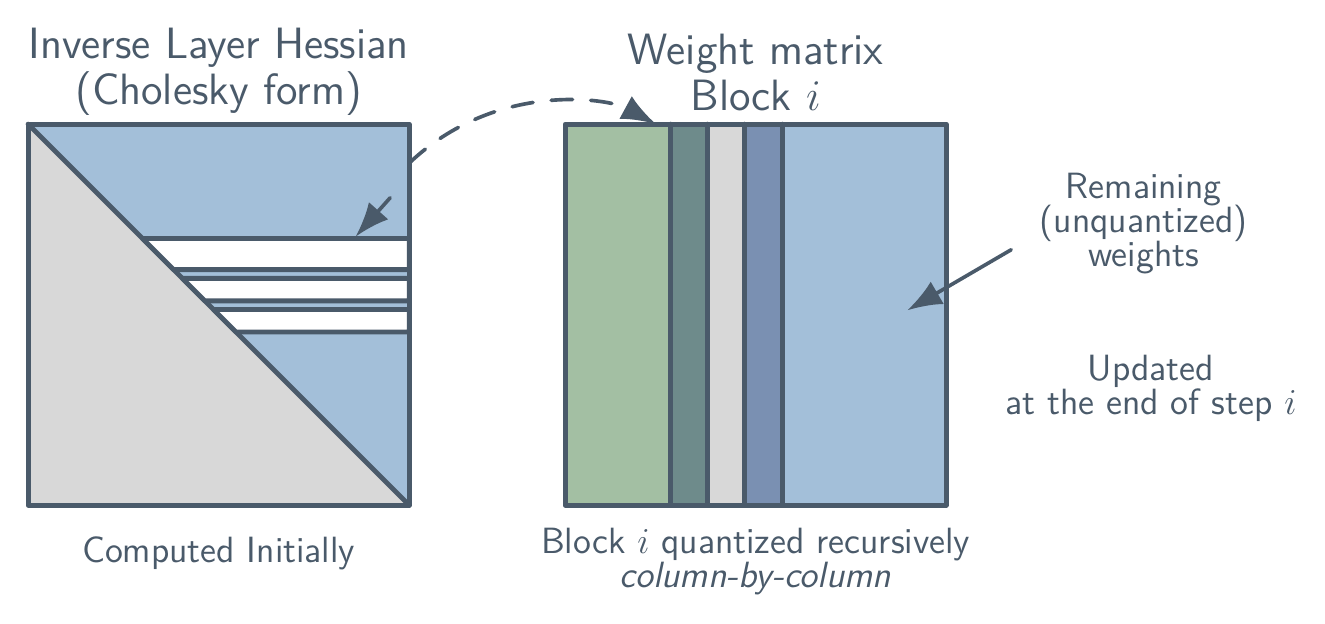
\includegraphics[width=0.98\textwidth,height=0.72\textheight,keepaspectratio]{figures/compression/gptq_pipeline.png}%
}
\caption[GPTQ algorithm]{\small The GPTQ Algorithm. To avoid computationally prohibitive row-wise updates of OBQ, GPTQ employs a Lazy Batch-Update strategy, quantizing weights in blocks. \cite{frantar2022gptq}}
\label{fig:gptq}
\end{figure}

GPTQ scales second-order quantization to billion-parameter models by building upon Optimal Brain Quantization (OBQ) while introducing three critical algorithmic innovations that reduce complexity from months to hours. While OBQ provides high-accuracy quantization through Hessian-based error correction, its $O(d_{\text{row}}\cdot d_{\text{col}}^{3})$ complexity renders it infeasible for LLMs. Standard Round-to-Nearest (RTN) executes quickly but destroys accuracy. GPTQ bridges this gap by approximating second-order optimization with runtime comparable to a single forward pass.

\paragraph{Methodology.}
GPTQ solves the layer-wise reconstruction problem:
\begin{equation}
\hat{\bm{W}} \;=\; \arg\min_{\tilde{\bm{W}}} \, \| \bm{W}\bm{X} - \tilde{\bm{W}}\bm{X} \|_{F}^{2}
\end{equation}
Using trace identities, this becomes:
\begin{equation}
\| \bm{W}\bm{X} - \tilde{\bm{W}}\bm{X} \|_{F}^{2} \;=\; \operatorname{Tr}\!\big( (\bm{W}-\tilde{\bm{W}})\,\bm{X}\bm{X}^\top(\bm{W}-\tilde{\bm{W}})^\top \big)
\end{equation}
For a single row $\bm{w}$, the Hessian is $\bm{H} = 2\,\bm{X}\bm{X}^\top$, yielding quadratic form:
\begin{equation}
\ell(\tilde{\bm{w}}) \;=\; \tfrac{1}{2}\,(\bm{w}-\tilde{\bm{w}})^\top \bm{H} (\bm{w}-\tilde{\bm{w}})
\end{equation}

\methoddetail{Algorithm Overview}
GPTQ rounds the columns of $\bm{W}$ one at a time, from left to right. Before it begins, it builds the inverse Hessian $\bm{H}^{-1}=(2\bm{X}\bm{X}^\top+\lambda\bm{I})^{-1}$ from the calibration inputs $\bm{X}$, where $\lambda$ is a small constant added to the diagonal for stability; this matrix tells it how to adjust the columns it has not yet touched whenever it rounds one. After rounding column $j$ to the low-bit grid, GPTQ measures the error this caused and pushes a matching correction onto the remaining columns:
\begin{equation}
  \bm{e}_j = \frac{\bm{W}_{:,j} - \operatorname{quant}(\bm{W}_{:,j})}{[\bm{H}^{-1}]_{jj}},
  \qquad
  \bm{W}_{:,\,j+1:} \;\leftarrow\; \bm{W}_{:,\,j+1:} - \bm{e}_j\,\bm{H}^{-1}_{j,\,j+1:},
  \label{eq:gptq_update}
\end{equation}
where $\bm{e}_j$ is the rounding error of column $j$ divided by the diagonal entry $[\bm{H}^{-1}]_{jj}$, and $\bm{H}^{-1}_{j,\,j+1:}$ is the part of row $j$ that sets how strongly each later column is corrected. To keep the GPU busy, these corrections are confined to a block of $B$ columns (typically $B = 128$) while the block is processed, and only once the block is finished is its accumulated error applied to all columns that follow. The inverse Hessian is prepared once through a Cholesky factorization, which keeps the repeated corrections numerically stable on large matrices.

\paragraph{Key Properties and Results.}
GPTQ reduces OBQ runtime by orders of magnitude through shared column ordering, block updates, and Cholesky precomputation. Complexity decreases from $O(d_{\text{row}}\cdot d_{\text{col}}^{3})$ to $O\!\big(\max\{d_{\text{row}}\cdot d_{\text{col}}^{2},\, d_{\text{col}}^{3}\}\big)$ in practice. The method quantizes OPT-175B to 3–4 bits with negligible perplexity degradation in $\approx 4 $  GPU hours (single A100) using 128 calibration samples. It supports flexible bit-widths (4/3/2-bit, with 2-bit typically requiring smaller blocks) and operates as pure post-training quantization requiring minimal calibration data.

\subsubsection{VPTQ \cite{liu2024vptq}}

\begin{figure}[H]
\centering
\makebox[\textwidth][c]{%
  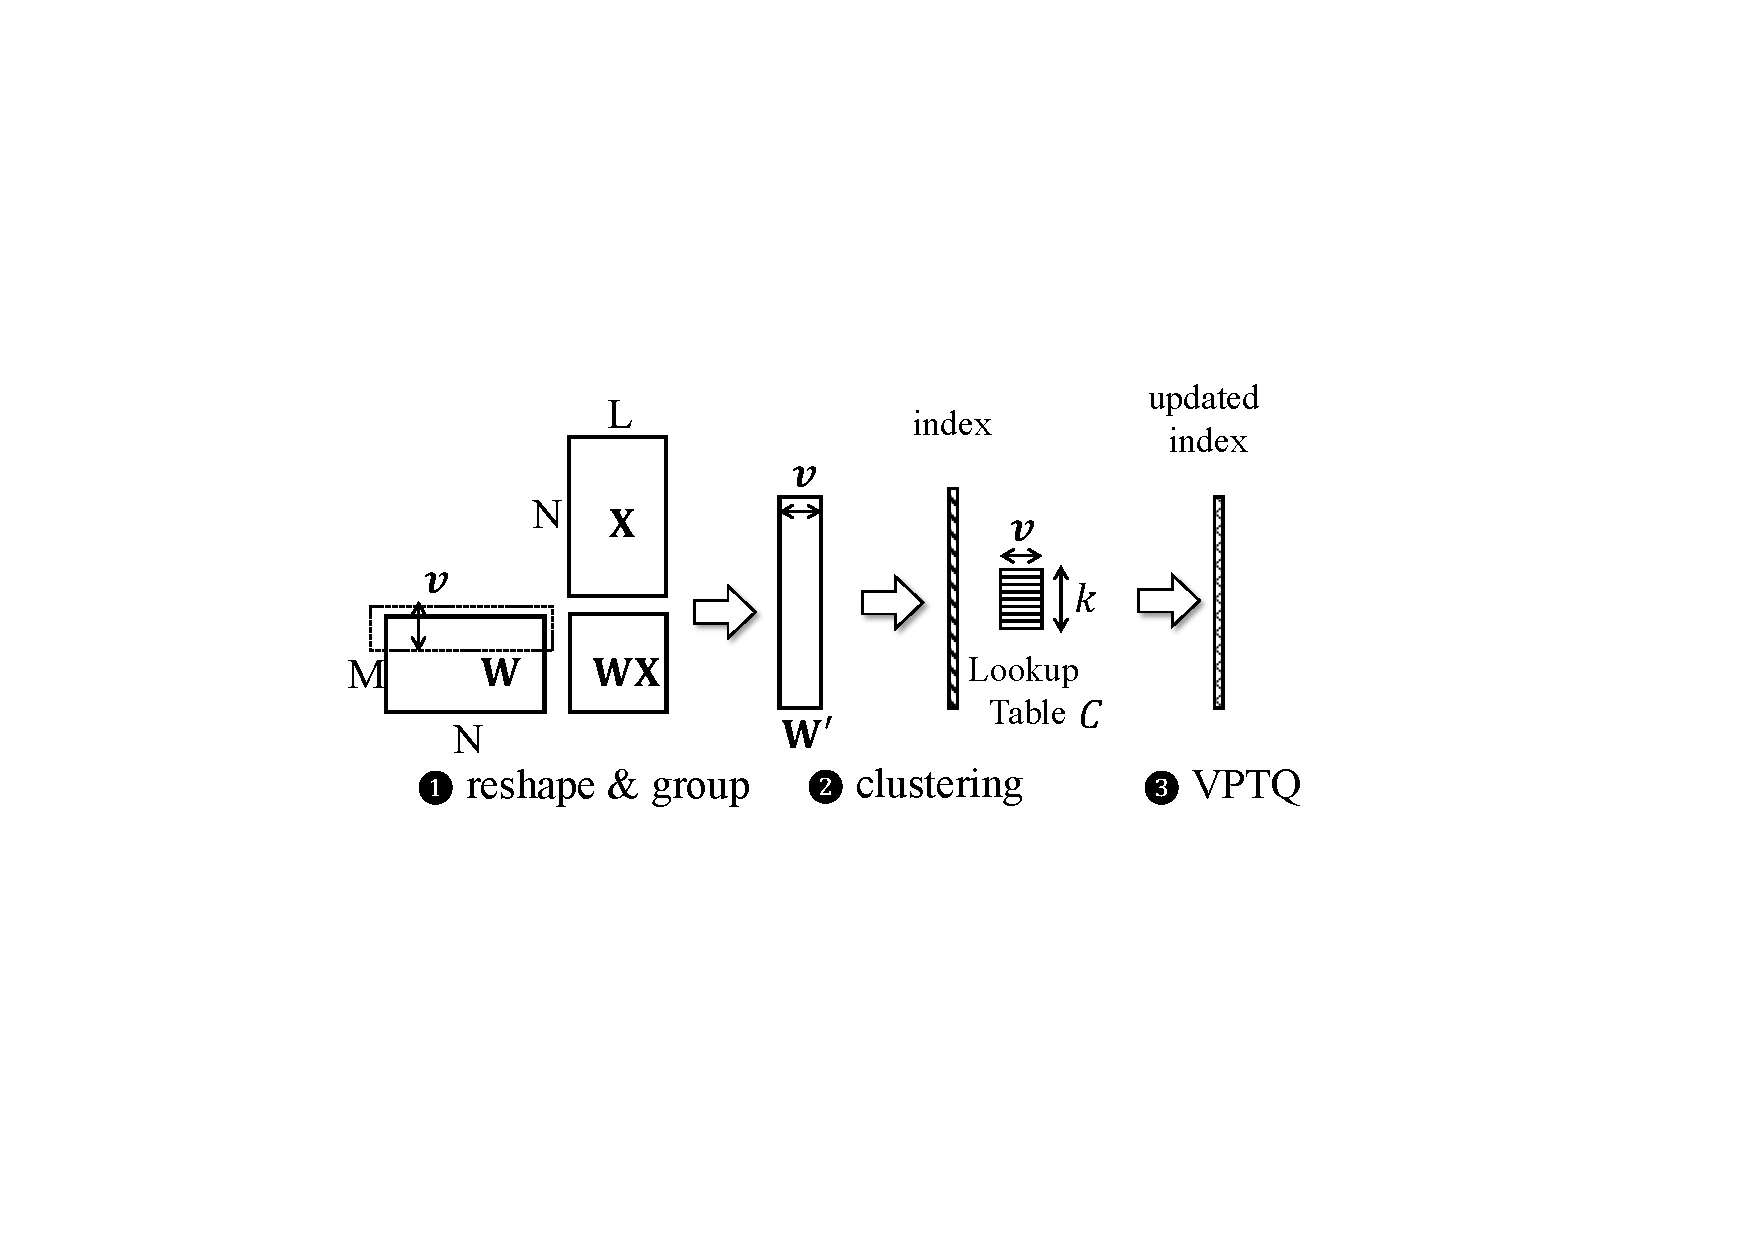
\includegraphics[width=0.72\textwidth,height=0.42\textheight,keepaspectratio]{figures/compression/vptq_methodology.pdf}%
}
\caption[VPTQ methodology]{VPTQ partitions weights into short vectors represented by centroid indices and codebooks. Quantization uses column-wise second-order updates, and inference reconstructs weights through lookup-table reads. \cite{liu2024vptq}}
\label{fig:vptq}
\end{figure}

VPTQ (Vector Post-Training Quantization) targets the regime where scalar weight-only PTQ becomes unstable near $2$ effective bits. Instead of rounding each scalar independently, it partitions each weight column into short vectors $\bm{v}_{j,t} \in \mathbb{R}^{\ell}$ and represents each vector by an index into a learned codebook $\mathcal{C} = \{\bm{c}_1,\dots,\bm{c}_K\}$, enabling fractional effective bit-widths and capturing correlations among neighboring weights.

\paragraph{Methodology.}
The quantization objective is the standard second-order PTQ proxy:
\begin{equation}
\min_{\hat{\bm{W}} \in \mathcal{Q}}
  \operatorname{Tr}\!\bigl((\bm{W}-\hat{\bm{W}})\,\bm{H}\,(\bm{W}-\hat{\bm{W}})^\top\bigr),
\end{equation}
where $\bm{H}$ is the layer Hessian estimated from calibration data and $\mathcal{Q}$ is the set of vector-quantized matrices. Columns are processed one at a time: after assigning column $j$, the error $\bm{\delta}_j = \bm{w}_j - \hat{\bm{w}}_j$ propagates to the remaining unquantized columns $F$ via
\begin{equation}
\bm{W}_{:,F} \leftarrow \bm{W}_{:,F}
  - \frac{\bm{\delta}_j}{[\bm{H}^{-1}]_{jj}}\,[\bm{H}^{-1}]_{jF},
\end{equation}
the same GPTQ-style correction that prevents error accumulation across columns. The codebook is initialized by solving a Hessian-weighted $k$-means over the weight vectors $\{\bm{v}_{j,t}\}$:
\begin{equation}
\min_{\mathcal{C},\mathcal{I}}
  \sum_{j,t} h_{j,t}\,\|\bm{v}_{j,t} - \bm{c}_{I_{j,t}}\|_2^2,
\end{equation}
where $h_{j,t}$ is the local Hessian weight for vector $(j,t)$; vectors in high-curvature directions of the reconstruction loss pull centroids harder, seeding the codebook toward the weight patterns that matter most for output fidelity. A second codebook is then fitted to the residuals $\bm{r}_{j,t} = \bm{v}_{j,t} - \bm{c}^{(1)}_{I_{j,t}}$, so each vector is represented by two indices rather than one, recovering precision without widening the primary codebook. Outlier-dominated tiles are assigned a separate partition. At inference, weights are reconstructed entirely by lookup-table reads on the stored indices and codebooks.

\methoddetail{Algorithm Overview}{
  VPTQ proceeds layer by layer.
  (1)~Compute the layer Hessian $\bm{H}$ from calibration activations and partition each weight column into vectors $\{\bm{v}_{j,t}\}$ of length $\ell$.
  (2)~Initialize the primary codebook $\mathcal{C}^{(1)}$ via Hessian-weighted $k$-means over $\{\bm{v}_{j,t}\}$, using $h_{j,t}$ as per-vector weights.
  (3)~Quantize columns left to right: assign each $\bm{v}_{j,t}$ to its nearest centroid, accumulate the column error $\bm{\delta}_j$, and propagate it to all remaining columns via the inverse-Hessian update.
  (4)~Fit a residual codebook $\mathcal{C}^{(2)}$ to the first-stage residuals $\{\bm{r}_{j,t}\}$; assign outlier-dominated tiles to a dedicated partition.
  (5)~Store the layer as centroid index pairs plus codebooks; inference reconstructs weights by lookup rather than dequantization arithmetic.
}

\paragraph{Results.}
VPTQ reaches ${\approx}2.02$ effective bits on LLaMA-2-7B (WikiText-2 PPL~$6.13$, AvgQA~$58.2$) and LLaMA-3-70B (PPL~$5.60$, AvgQA~$70.9$) \cite{liu2024vptq}, with a $1.6$--$1.8\times$ throughput gain over prior ultra-low-bit baselines attributed to lookup-based decoding and vector lengths aligned with cache-line granularity.

\subsection{Optimization-Based Methods}

Compensation-based methods repair rounding error with a fixed rule read off the curvature. The next family is less committed: instead of fixing the error afterwards, it treats the quantizer's own settings as quantities to be learned. Optimization-based post-training quantization casts the design of quantizer as a calibration problem. The default approach in PTQ to determine the quantized value for a weight or activation involves the simple mapping of translating the range of real values (determined using calibration data) into a scale factor and then rounding all values to the nearest integer. These choices are quick, but localized and static; one large activation can significantly inflate the quantization range and the same rounding mechanism may be used when rounding up versus rounding down produce differing impacts on the output, and the bit precision allocated to a layer may not directly reflect the optimization of reconstruction error.

Therefore, optimization-based methods started to appear as substitutes for these hand-crafted choices by treating them as variables that are tuned on a small calibration set. While the full precision model is fixed, the quantization setup is changed in order to minimize the discrepancy between the full-precision and the quantized model. Depending on the strategy, optimized variables may include rounding, clipping ranges, scaling factors, equivalent transformations, layer-wise precision selection. Since quantization involves discrete operations, particularly rounding, these strategies mostly used continuous relaxation or straight-through gradient estimations to allow the optimization by backpropagation\cite{nagel2020adaround,li2021brecq,esser2020learned,shao2024omniquant}.

\subsubsection{OmniQuant \cite{shao2024omniquant}}

\begin{figure}[htbp]
\centering
\makebox[\textwidth][c]{%
  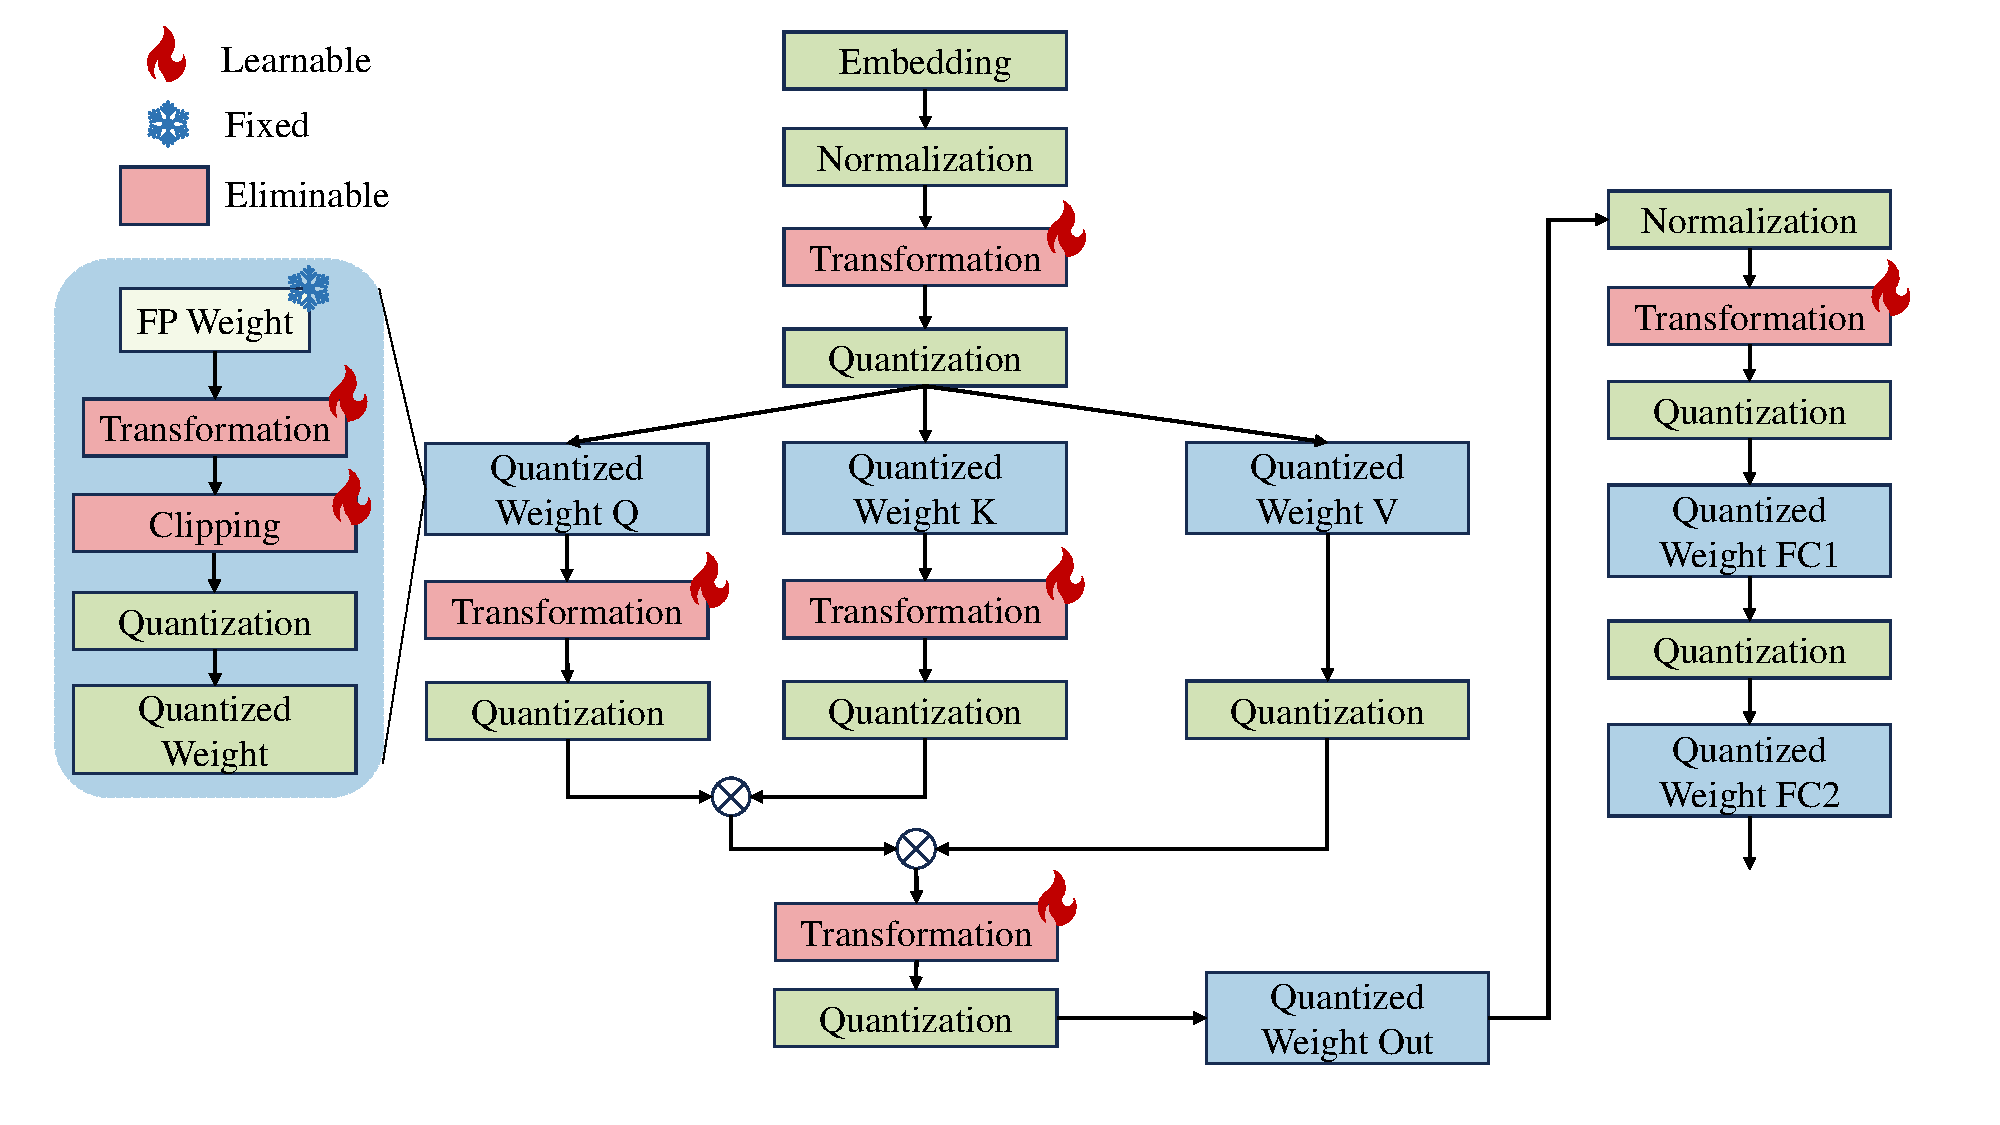
\includegraphics[width=0.98\textwidth,height=0.72\textheight,keepaspectratio]{figures/compression/omniquant_framework.pdf}%
}
\caption[OmniQuant methodology]{OmniQuant freezes the original full-precision weights and learns quantization parameters via gradient descent, simultaneously optimizing Learnable Weight Clipping (LWC) and Learnable Equivalent Transformation (LET). All learnable parameters are absorbed into the quantized weights after calibration, introducing no runtime overhead.}
\label{fig:omniquant}
\end{figure}

\paragraph{Methodology.}
OmniQuant freezes the original full-precision weights and optimizes a small set of learnable quantization parameters through block-wise gradient descent on a calibration set. Processing one block at a time keeps the optimization tractable without retraining the full model.

The first component, Learnable Weight Clipping (LWC), replaces fixed range estimation with learnable upper and lower clipping strengths $\gamma, \beta \in [0,1]$, parameterized via sigmoid. Given a weight matrix $\mathbf{W}$, a target bit-width $N$, and a zero-point $z$ that aligns real zero to an integer code, the step size is $h = (\gamma\max(\mathbf{W}) - \beta\min(\mathbf{W}))/(2^N - 1)$, where $\max(\mathbf{W})$ and $\min(\mathbf{W})$ are the maximum and minimum values of the weight matrix. The quantized weight is then:
\begin{equation}
\mathbf{W}_q = \text{clamp}\!\left(\left\lfloor\frac{\mathbf{W}}{h}\right\rfloor + z,\; 0,\; 2^N - 1\right)
\end{equation}
When $\gamma = \beta = 1$, $h$ reduces to the standard MinMax step size — the range divided uniformly into $2^N - 1$ levels — so LWC strictly generalizes that baseline.

The second component, Learnable Equivalent Transformation (LET), addresses activation outliers by learning a channel-wise scaling vector $\mathbf{s} \in \mathbb{R}^{C_{in}}$ and shifting vector $\delta \in \mathbb{R}^{C_{in}}$, where $C_{in}$ is the number of input channels. These produce a mathematically equivalent rearrangement of the linear layer $\mathbf{Y} = \mathbf{X}\mathbf{W} + \mathbf{B}$:
\begin{equation}
\mathbf{Y} = \underbrace{[(\mathbf{X} - \delta) \oslash \mathbf{s}]}_{\tilde{\mathbf{X}}} \cdot \underbrace{[\mathbf{s} \odot \mathbf{W}]}_{\tilde{\mathbf{W}}} + \underbrace{[\mathbf{B} + \delta\mathbf{W}]}_{\tilde{\mathbf{B}}}
\end{equation}
where $\oslash$ and $\odot$ denote elementwise division and multiplication respectively. The transformed activation $\tilde{\mathbf{X}}$ is quantization-friendly since the outlier magnitude has been shifted into $\tilde{\mathbf{W}}$, where LWC handles it. After calibration, $\mathbf{s}$ and $\delta$ are absorbed into adjacent weights, adding no runtime overhead.

Both components are optimized jointly by minimizing the squared output mismatch between the original and quantized block:
\begin{equation}
\arg\min_{\Theta_1, \Theta_2} \left\|\mathcal{F}(\mathbf{W}, \mathbf{X}) - \mathcal{F}\!\left(Q_w(\mathbf{W};\,\Theta_1,\Theta_2),\; Q_a(\mathbf{X};\,\Theta_2)\right)\right\|
\label{eq:omniquant_obj}
\end{equation}
where $\mathcal{F}$ is the forward mapping of one transformer block, $Q_w$ and $Q_a$ are the weight and activation quantizers, and $\Theta_1 = \{\gamma,\beta\}$, $\Theta_2 = \{\mathbf{s},\delta\}$ are the LWC and LET parameters. SGD with straight-through estimation handles the non-differentiable rounding.

\methoddetail{Algorithm Overview}
OmniQuant calibrates one transformer block at a time and never changes the original weights, which keeps the procedure light enough to run on a single GPU. For each block it starts the clipping strengths $\gamma,\beta$ and the scaling and shifting vectors $\mathbf{s},\delta$ at their neutral values, then repeats the following for a few epochs over the calibration set: it applies the current LET transform and the current LWC quantizer to the block, sends the calibration inputs through both the original block and this quantized version, and takes a gradient step on $\gamma,\beta,\mathbf{s},\delta$ to shrink the squared difference between the two outputs (Eq.~\ref{eq:omniquant_obj}). Since rounding has no usable gradient, a straight-through estimator passes the gradient through it unchanged. Once the block is calibrated, the learned $\mathbf{s}$ and $\delta$ are merged into the neighbouring weights and the block is quantized for good; its quantized output then serves as the input for calibrating the next block.

\paragraph{Results.}
On weight-only quantization, the gains are most pronounced at low bit-widths. At W2A16 on LLaMA-1-13B, OmniQuant achieves a WikiText-2 perplexity of 13.21 while GPTQ collapses to 3832. At W2A16 on LLaMA-1-7B, OmniQuant reaches 15.47 against RTN at $1.1 \times 10^5$. At higher bit-widths the margins narrow: at W3A16 on LLaMA-1-7B OmniQuant reaches 6.49 and at W4A16 it reaches 5.86, consistently ahead of prior methods across the full LLaMA-1 and LLaMA-2 families.

On weight-activation quantization at W4A4, OmniQuant achieves 52.65\% average zero-shot accuracy on LLaMA-1-7B across six tasks, against 48.43\% for the best prior PTQ method and 46.43\% for LLM-QAT+SQ, which requires quantization-aware training with 100k samples. The LLaMA-2 family from 7B to 70B is processed on a single A100-40G GPU with 128 calibration samples in 1 to 16 hours.

\subsection{Search-Based Methods}

The methods reviewed so far assign bit-widths layer by layer using local importance scores or learned parameters, implicitly assuming that a lower sum of per-layer quantization errors produces a better model overall. A different perspective treats the per-layer bit-width assignment as a combinatorial optimization problem and searches over the space of valid configurations directly. This avoids the error-monotonicity assumption entirely: rather than scoring layers independently and minimizing a linear sum, search-based methods evaluate complete compressed models and select the configuration that minimizes end-to-end output degradation subject to a compression budget.

\subsubsection{EvoPress \cite{evopress2024}}

\paragraph{Methodology.}
For quantization, EvoPress first builds a level database by compressing each linear layer independently to each available bit-width (2, 3, 4, 5, and 6 bits) using GPTQ with group size 128. A compressed model is then a vector $v \in \{2,3,4,5,6\}^n$ assigning one bit-width to each of the $n$ layers. The search objective is:
\begin{equation}
  \hat{M}^* = \operatorname{arg\,min}_{v} \; D_{\mathrm{KL}}
    \bigl(P_M \;\|\; Q_{\hat{M}_v}\bigr)
    \quad \text{subject to} \quad
    \mathrm{size}(\hat{M}_v) \leq C,
\end{equation}
where $P_M$ and $Q_{\hat{M}_v}$ are the output distributions of the original and compressed model on calibration tokens, and $C$ is the target model size. KL divergence is used as the fitness signal rather than perplexity or layer-wise MSE, as it is more robust under limited calibration data.

The search follows a $(1+\lambda)$-evolutionary algorithm with level-switch mutation: one layer's bit-width is raised by one step while a second layer of the same size has its bit-width lowered by one step, preserving the compression budget exactly. Selection uses aggressive multi-step evaluation: all $\lambda$ offspring are first scored on a fraction of a calibration batch, the weakest candidates are eliminated, and the survivors are re-evaluated on progressively larger batches, reaching a full minibatch only in the final stage.

\methoddetail{Algorithm Overview}{
  (1)~Build the level database: compress each layer to each available bit-width with GPTQ (group size 128).
  (2)~Initialize with the uniform assignment at the target average bit-width.
  (3)~Each generation: generate $\lambda$ offspring via level-switch mutation (raise one layer by one bit, lower a same-size layer by one bit).
  (4)~Evaluate offspring in multiple stages with increasing token budgets; retain only the fittest at each stage.
  (5)~Repeat until convergence; the survivor defines the per-layer bit-width profile applied at inference.
}

\paragraph{Results.}
At 3-bit average quantization on Llama-3-8B, EvoPress achieves WikiText-2 PPL~7.49 against uniform GPTQ PPL~12.19 and DP-based search PPL~29.00, with zero-shot average accuracy 64.3 versus 60.2 for uniform. The collapse of DP to PPL~29.00 on the same model illustrates precisely why error monotonicity fails at extreme compression: minimizing a linear sum of layer-wise errors selects a configuration that is locally cheap but globally destructive. On Mistral-7B-v0.3 the gap is more modest (PPL~5.21 vs~5.54) but consistent across all tested models. EvoPress also supports hardware-aware constrained search: under vLLM's restriction to 4-bit and 8-bit only with shared bit-widths inside each block, it finds mixed-precision profiles that preserve accuracy at the same average bit-width.

\subsection{Empirical Comparison}

The comparison is organized around three compression scenarios. The first is weight-only quantization across the 4-, 3-, and 2-bit spectrum, where the dominant variable is the quantization family. The second is joint weight-and-activation quantization at 4 bits (W4A4), which additionally requires controlling dynamic activation distributions at inference time. The third is non-uniform bit-width search, where the allocation of bits across layers is itself the optimization target. Perplexity (PPL) on WikiText-2 is the primary metric ($\downarrow$ better); zero-shot average accuracy on reasoning benchmarks is used as a secondary metric ($\uparrow$ better) where reported.

Table~\ref{tab:ptq-taxonomy} summarizes the methods reviewed in this section by the dominant mechanism used to control quantization error.

\begin{table}[htbp]
\centering
\caption[PTQ methods by family]{Methods covered in this section, organized by error-control family.}
\label{tab:ptq-taxonomy}
\begin{tabular}{lllp{7.5cm}}
  \toprule
  \textbf{Method} & \textbf{Family} & \textbf{Quantizes} & \textbf{Key mechanism} \\
  \midrule
  GPTQ      & Compensation         & Weights      & Second-order layer-wise reconstruction via OBS \\
  QuIP      & Rotation + Comp.     & Weights      & Incoherence via orthogonal transforms; LDLQ coordinate descent \\
  VPTQ      & Compensation         & Weights      & Hessian-weighted vector quantization with residual codebook \\
  QuaRot    & Rotation             & W + Act      & Hadamard rotation fused into the model for outlier removal \\
  OWQ       & Salience             & Weights      & Mixed-precision via activation-outlier column detection \\
  OmniQuant & Optimization         & Weights      & Learnable equivalent transformation optimized on calibration data \\
  EvoPress  & Search               & Weights      & Evolutionary search over per-layer bit-width profiles under a size budget \\
  \bottomrule
\end{tabular}
\end{table}

GPTQ, QuIP, and VPTQ cover the weight-only spectrum from 4 bits down to 2 bits; OmniQuant spans the same range through a learned transformation rather than second-order correction. Table~\ref{tab:weight-only-spectrum} reports WikiText-2 perplexity on LLaMA-3-8B and LLaMA-3-70B for the three compensation- and rotation-based methods. OmniQuant results, evaluated by the original authors on LLaMA-2-7B and LLaMA-2-70B (comparable scale, one generation earlier), are included with a footnote to indicate the architecture difference.

\begin{table}[htbp]
\centering
\caption[Weight-only quantization spectrum]{WikiText-2 perplexity ($\downarrow$) for weight-only quantization across bit-width regimes. GPTQ at 2 bits without grouping produces perplexity in the thousands and is omitted from that block.}
\label{tab:weight-only-spectrum}
\begin{tabular}{llcc}
  \toprule
  \textbf{Method} & \textbf{Bits} & \textbf{8B model} & \textbf{70B model} \\
  \midrule
  FP16 & 16 & 6.14 & 2.90 \\
  \midrule
  \multicolumn{4}{l}{\textit{4-bit weight-only}} \\
  GPTQ                & 4            & 6.50 & 3.30 \\
  QuIP                & 4            & 6.50 & 3.40 \\
  VPTQ                & $\approx$4   & 6.42 & 3.15 \\
  OmniQuant\textsuperscript{$\dagger$} & 4 & 5.74 & 3.47 \\
  \midrule
  \multicolumn{4}{l}{\textit{3-bit weight-only}} \\
  GPTQ                & 3            & 8.20 & 5.20 \\
  QuIP                & 3            & 7.50 & 4.70 \\
  VPTQ                & $\approx$3   & 6.97 & 3.81 \\
  OmniQuant\textsuperscript{$\dagger$} & 3 & 6.58 & 3.92 \\
  \midrule
  \multicolumn{4}{l}{\textit{2-bit weight-only}} \\
  VPTQ                & $\approx$2   & 5.64 & 5.66 \\
  OmniQuant\textsuperscript{$\dagger$} & 2 (g128) & 11.06 & 6.55 \\
  \bottomrule
  \multicolumn{4}{l}{\footnotesize\textsuperscript{$\dagger$}OmniQuant evaluated on LLaMA-2-7B / LLaMA-2-70B; GPTQ, QuIP, VPTQ on LLaMA-3-8B / LLaMA-3-70B.}
\end{tabular}
\end{table}

Joint quantization of both weights and activations to 4 bits (W4A4) is a stricter regime: activation values vary at inference time and cannot be pre-compensated by a static calibration pass. Table~\ref{tab:w4a4-comparison} compares SmoothQuant (the channel-rescaling baseline), OmniQuant (optimization-based), and QuaRot (rotation-based preprocessing) on WikiText-2. AffineQ, QLLM, and Atom are not covered in this section and are omitted.

\begin{table}[htbp]
\centering
\caption[W4A4 perplexity comparison]{WikiText-2 perplexity ($\downarrow$) under W4A4 joint quantization on LLaMA-1 and LLaMA-2. QuaRot results use the GPTQ rounding variant (QR-GPTQ); dashes indicate the model was not evaluated in that work.}
\label{tab:w4a4-comparison}
\begin{tabular}{lcccc}
  \toprule
  & \multicolumn{2}{c}{\textbf{LLaMA-1}} & \multicolumn{2}{c}{\textbf{LLaMA-2}} \\
  \textbf{Method} & \textbf{7B} & \textbf{13B} & \textbf{7B} & \textbf{13B} \\
  \midrule
  FP16        & 5.68 & 5.09 & 5.47 & 4.88 \\
  \midrule
  SmoothQuant & 25.2 & 40.0 & 83.1 & 35.8 \\
  OmniQuant   & \textbf{11.2} & \textbf{10.8} & 14.2 & 12.3 \\
  QuaRot      & —    & —    & \textbf{6.10} & \textbf{5.40} \\
  \bottomrule
\end{tabular}
\end{table}

Non-uniform bit-width search assigns a distinct compression level to each layer rather than applying a single bit-width uniformly. This allows layers with higher sensitivity to retain more bits at the expense of less-sensitive layers, without increasing the total model size. Table~\ref{tab:evopress-search} shows results for EvoPress against two baselines at a target average of 3 bits: uniform GPTQ (all layers at the same bit-width) and a dynamic-programming search that greedily minimizes the sum of per-layer GPTQ reconstruction errors.

\begin{table}[htbp]
\centering
\caption[EvoPress non-uniform quantization results]{WikiText-2 PPL ($\downarrow$) and zero-shot average accuracy ($\uparrow$) at $\sim$3-bit average weight quantization. DP minimizes the sum of layer-wise GPTQ errors; EvoPress minimizes end-to-end KL divergence from the original model. A dash indicates the result was not reported for that model.}
\label{tab:evopress-search}
\begin{tabular}{lcccccc}
  \toprule
  & \multicolumn{3}{c}{\textbf{WikiText-2 PPL} $\downarrow$} & \multicolumn{3}{c}{\textbf{Zero-shot Avg.} $\uparrow$} \\
  \textbf{Model} & \textbf{Uniform} & \textbf{DP} & \textbf{EvoPress} & \textbf{Uniform} & \textbf{DP} & \textbf{EvoPress} \\
  \midrule
  Mistral-7B  & 5.54  & —     & \textbf{5.21} & — & — & — \\
  LLaMA-3-8B  & 12.19 & 29.00 & \textbf{7.49} & 60.2 & — & \textbf{64.3} \\
  \bottomrule
\end{tabular}
\end{table}

At 4-bit weight-only quantization, second-order compensation (GPTQ) already recovers most of the full-precision accuracy gap, and vector quantization (VPTQ) extends this advantage to 3 bits and remains functional at 2 bits where scalar methods require very small group sizes to avoid collapse. Enabling activation quantization (W4A4) introduces a qualitatively distinct challenge: SmoothQuant's channel-wise rescaling leaves large perplexity gaps, OmniQuant's learned transformation improves upon it, but rotation-based preprocessing (QuaRot) is the only family that approaches near-lossless results in this regime. Non-uniform search (EvoPress) provides an orthogonal gain: at the same average bit-width, it outperforms both uniform assignment and DP-based layer scoring, with the advantage widening dramatically at extreme compression where the error-monotonicity assumption underlying DP fails catastrophically.


\newpage
\input{sections/compression/pruning_methods}
% !TEX root = ../../main_without_quantization.tex
\section{Discussion}
\label{sec:discussion}

\subsection{Local scoring and its limits}
\label{subsec:local_scores_configuration_choices}

The reviewed methods show a clear progression in what is being scored. Magnitude pruning assigns importance through the absolute weight value $|W_{i,j}|$ alone, a criterion that carries no information about how actively each weight contributes to the model output. Applied to large language models, this proves insufficient: Sun et al.\ report that magnitude-based selection fails severely even at relatively low sparsity levels \cite{sun2023simple}, and Ma et al.\ observe that pruning ratios above roughly 20\% trigger a rapid representational collapse under magnitude scoring \cite{ma2023llmpruner}. The perplexity results in Table~\ref{tab:unsupported_comparison} confirm this directly: on LLaMA-7B at 50\% unstructured sparsity, magnitude pruning raises perplexity from 5.68 to 17.29. Wanda addresses this by incorporating the activation norm of the coupled input channel into the saliency score, so that a weight receives higher importance when its input direction is consistently active across calibration samples \cite{sun2023simple}. SparseGPT replaces the magnitude surrogate with a second-order compensation term derived from a block-wise Hessian approximation, applied locally after each weight removal to counteract the induced output error \cite{frantar2023sparsegpt}. Both methods substantially narrow the gap: SparseGPT gives 7.22 and Wanda gives 7.26 on LLaMA-7B at 50\% sparsity (Table~\ref{tab:unsupported_comparison}), with a consistent ordering on LLaMA-13B where magnitude reaches 20.21 against SparseGPT at 6.21 and Wanda at 6.15 \cite{frantar2023sparsegpt,sun2023simple}. Across both models, the evidence supports a specific conclusion: for weight-level pruning of large language models, a saliency criterion must account for activation statistics or output curvature rather than weight magnitude in isolation.

The semi-structured results add another constraint. SparseGPT at 2:4 sparsity gives 12.96 perplexity on OPT-13B, 10.90 on OPT-30B, 10.09 on OPT-66B, and 8.74 on OPT-175B, against dense baselines of 10.13, 9.56, 9.34, and 8.35 respectively \cite{frantar2023sparsegpt}. The absolute penalty decreases with model scale, but the 2:4 constraint consistently exceeds the cost of unconstrained unstructured pruning at the same nominal sparsity (Table~\ref{tab:unsupported_comparison}). This is why MRP treats the removed N:M group jointly rather than applying single-weight compensation repeatedly \cite{zhao2024pruning}. The point is not that MRP replaces SparseGPT in every setting. It handles a case where the feasible mask itself couples the removed weights.

\subsection{Structured pruning as architecture selection}
\label{subsec:structured_pruning_architecture_selection}

Once pruning moves to heads, FFN channels, hidden dimensions, or layers, the decision is no longer only about individual weights. LLM-Pruner first builds dependency groups so that the removed structures remain consistent with the model graph \cite{ma2023llmpruner}. CoFi learns masks over several Transformer structures at once, including attention blocks, heads, FFN blocks, intermediate channels, and hidden dimensions \cite{xia2022cofi}. Fast post-training pruning uses Fisher-based scores under FLOPs or latency constraints \cite{kwon2022fast}. ZipLM applies second-order scoring to executable Transformer structures and adds measured runtime information during search \cite{kurtic2023ziplm}.

The reported structured results match this shift in object. LLM-Pruner keeps 98.6\% zero-shot accuracy retention at a 20\% prune ratio on LLaMA-7B, but drops to 83.6\% retention at a 50\% prune ratio. CoFi reaches 80.6 MNLI accuracy at about $12\times$ speedup, compared with 78.8 for TinyBERT$_4$ at a similar speedup, and reaches 82.6 F1 on SQuADv1 at about $8.7\times$ speedup. Fast post-training pruning reports 60--70\% remaining FLOPs with at most a 1\% accuracy or F1 drop on GLUE and SQuAD, together with measured latency speedups of $1.34\times$ at batch size 32 and $1.47\times$ at batch size 256 \cite{kwon2022fast}. ZipLM reports 91.4/84.8 accuracy on QNLI/MNLI at $2\times$ speedup for BERT Base, then 88.6/82.7 at $10\times$ speedup with roughly 5M parameters. These results are not just better or worse versions of weight pruning. They are pruning results over executable model structure.

Structured pruning also makes the search space more coupled. Removing one head, layer, or intermediate dimension changes the role of nearby structures, and a uniform allocation across the network is rarely optimal. DarwinLM frames this directly: different model components exhibit different sensitivities to pruning, which motivates non-uniform structured compression and a training-aware search over candidate architectures \cite{darwinlm2025}. The implication is that the best allocation is a property of the full configuration, not of any single removable unit scored in isolation.

\subsection{Why global allocation remains unresolved}
\label{subsec:local_ranking_high_compression}

A constraint that is common to all these techniques is that of allocation. We notice that while techniques like Wanda and SparseGPT demonstrate how much weight level pruning can be augmented with the help of activation information, or second order compensation \cite{sun2023simple,frantar2023sparsegpt}, the issue here is that these scores still only represent locally the impact of removing individual weights, channels, heads or blocks before the whole architecture post compression is determined. A layer, for example, that is 'safe' to prune according to its score can still have a negative interaction with the decision to prune some other layer elsewhere, and a given layer can only be drastically compressed if capacity is conserved in the layers around it.

EvoPress formalises this observation by arguing that many dynamic compression methods rely on an assumption of error monotonicity, where the quality of a compressed model is expected to follow the sum of layer-wise compression errors \cite{evopress2024}. The authors show that this assumption need not hold for large language models: two compression profiles can have similar or even inverted local error sums while producing substantially different end-to-end behavior. This weakens the justification for a purely greedy or layer-wise allocation rule and motivates evaluating the realized effect of a complete profile rather than accumulating per-unit scores.

The empirical results make the scale of this effect visible. In depth pruning on Mistral-7B at 25\%, EvoPress gives 8.66 WikiText perplexity and 12.04 on C4, while ShortGPT gives 43.26 and 40.16, and Shortened LLaMA gives 14.94 and 19.30 \cite{evopress2024}. On Llama-2-7B at 37.5\% depth pruning, EvoPress gives 17.98/18.91 on WikiText/C4, compared with 70.94/63.51 for ShortGPT and 35.37/26.07 for Shortened LLaMA (Table~\ref{tab:search_summary}). These gaps are too big to just chalk up to local scoring formula differences. They indicate that the chosen mix of removed layers plays a major role in the outcome. The unstructured allocation results seem to point in the same direction but in a more moderate way: at 70\% sparsity on Mistral-7B, EvoPress achieves a 14.42 WikiText perplexity and a 53.8 task average, while uniform allocation hits 23.08 and 49.9 (Table~\ref{tab:search_summary}). Once the budget is split among layers, the way it’s allocated naturally impacts the quality of the candidates.

\subsection{Need for evolutionary search}
\label{subsec:evolutionary_search_need}

At high compression, the difficulty lies in finding the transformer's units allocation that keeps the remaining network usable, since a unit that appears safe under a local score may become damaging once other layers are also compressed around it, and since the quality of the compressed model is only observed after all layer decisions have been chosen togetherwe begin to see the evolutionary search becomes as a more useful framework although being usually more costly. in our case for example EvoPress represents each candidate as a vector of layer-wise compression ratios, mutates that vector under a fixed global budget, and evaluates the resulting allocation through KL-divergence against the reference model across progressively larger token budgets \cite{evopress2024}

The same candidate-level treatment appears in DarwinLM, where structured pruning is organized through a sparsity-level database built by OBS-style module pruning, then candidate models are assembled and are evaluated after a short fine-tuning stage, so the search acts on the full compressed architecture produced by the selected module configuration \cite{darwinlm2025}, and the reported comparison gives a useful indication of this role, since DarwinLM compresses Llama-2-7B into a $2{,}7$B model with $62{,}8$ average accuracy after 10B post-training tokens, close to the $62{,}6$ reported for ShearedLLaMA after 50B tokens in Table~\ref{tab:search_summary}, supports the use of search over complete candidate structures within the reported setting

This candidate-level formulation also makes the cost of the search explicit, since the number of possible profiles grows with the number of layers, removable structures, and admissible sparsity levels, and since each candidate has to be instantiated and measured, sometimes after partial training or fine-tuning, making fitness evaluation the dominant cost of the procedure, and making diversity harder to preserve when selection repeatedly amplifies structurally similar high-ranking candidates across generations \cite{cantupaz2000efficient,luque2011parallel}

From this point, the island model follows naturally as an organization of the same evolutionary process, since the population is divided into semi-independent subpopulations that evolve separately and exchange candidates only through periodic migration, allowing different islands to explore different regions of the pruning space before useful candidates are shared \cite{cantupaz2000efficient,luque2011parallel,meng2018dynamicisland}, and this structure also fits the computational shape of Transformer compression, since candidate evaluation carries most of the cost and can be distributed across workers, allowing the search to preserve architectural diversity and reduce wall-clock time while keeping evaluation centered on complete compressed models \cite{harada2021distributedpga}.


\section{Conclusion}
The literature reviewed in this chapter highlights a distinct shift in model compression: a move away from general-purpose reduction techniques toward architecture-specific optimizations tailored for the Transformer. While the fundamental goals remain constant, reducing memory footprint and latency, the presence of systematic activation outliers in Large Language Models has necessitated the development of specialized interventions such as rotation-based quantization and salience-aware protection.

The analysis suggests that quantization currently offers the most immediate path to deployment efficiency, particularly through methods that mitigate the precision loss caused by outlier channels. In contrast, while pruning offers high theoretical compression ratios, unstructured approaches face significant hurdles in translating parameter reduction into wall-clock speedup due to hardware incompatibility, and structured approaches trade compression depth for hardware compatibility.

